\documentclass[preprint,12pt,authoryear]{elsarticle}
\usepackage{amsmath,amssymb,booktabs,graphicx,textcomp,url}
\usepackage{tabularx,array,threeparttable}
\usepackage[most]{tcolorbox}

% Elsevier applies its own reference style after acceptance; at
% submission the format only has to be internally consistent.
\biboptions{round,authoryear}
\graphicspath{{figures/}{../figures/}}

% Float placement: without this the figures and tables drift to the
% end of the document and every \ref{} in the text points at a
\renewcommand{\topfraction}{0.9}
\renewcommand{\bottomfraction}{0.7}
\renewcommand{\textfraction}{0.07}
\renewcommand{\floatpagefraction}{0.85}
\setcounter{topnumber}{3}
\setcounter{bottomnumber}{2}
\setcounter{totalnumber}{5}

\journal{Ecological Informatics}

\begin{document}
\begin{frontmatter}

\title{Two axes of distribution shift in automated fern identification: image domain and geography, quantified on a 5,969-image, 152-species benchmark\tnotemark[1]}

\author[a,b]{Zihao Huang}
\ead{2309392013@st.gxu.edu.cn}
\author[a,b]{Yan Chen}
\ead{cy@gxu.edu.cn}
\author[c]{Yeming You}
\ead{youyeming@163.com}
\author[d]{Qi Zhang}
\ead{friendlyqi-work@foxmail.com}
\author[c]{Kai Su\corref{cor1}}
\ead{20210055@gxu.edu.cn}

\cortext[cor1]{Corresponding author.}

\address[a]{Guangxi Key Laboratory of Digital Infrastructure, Guangxi Zhuang Autonomous Region Information Center, Nanning 530000, China}
\address[b]{School of Computer and Electronic Information, Guangxi University, Nanning 530000, China}
\address[c]{Guangxi Colleges and Universities Key Laboratory for Cultivation and Utilization of Subtropical Forest Plantation, Key Laboratory of National Forestry and Grassland Administration on Cultivation of Fast-Growing Timber in Central South China, School of Forestry, Guangxi University, Nanning 530004, China}
\address[d]{China Post Group Co., Ltd. Nanning Branch, Nanning 530000, China}

\tnotetext[1]{Abbreviations: API, application programming interface; CC0 / CC BY / CC BY-NC, Creative Commons licences; CI, confidence interval; ECE, expected calibration error; GBIF, Global Biodiversity Information Facility; iDigBio, Integrated Digitized Biocollections; OCR, optical character recognition; pp, percentage points; PPG I, the Pteridophyte Phylogeny Group classification; VLM, vision--language model.}

\begin{abstract}
Automated species identification is increasingly proposed for ecological monitoring, yet its evaluation protocols routinely mix herbarium sheets with field photographs, ignore geographic provenance, and leave the accuracy of general-purpose vision--language models (VLMs) unaudited for text leakage. We present a fern benchmark of 5,969 images covering 152 species in 30 families from iNaturalist and GBIF, including iDigBio-digitised herbarium sheets. Every image records its image domain, data source and, after normalising 1,468 raw locality strings, country. It adds 700 open-set negatives in eight groups. Biology-pretrained features with a frozen trunk and a linear head at 336 px are the best recipe, at \textbf{91.4 $\pm$ 0.7\%} over three seeds. That is \textbf{+7.1 $\pm$ 1.0 pp} over DINOv2 in a paired comparison robust to seed variance, while a hierarchical head \emph{hurts} ($-$6.0 pp). Under this recipe, transferring across image domain or source costs \textbf{8.6--48.1 pp}, and leave-one-region-out geographic holdouts cost \textbf{3.6--39.8 pp}. The largest losses fall where test species have the least out-of-region training support (Spearman $\rho$ = 0.48, seven countries). Two independent VLMs reach only 24--32\% on a closed-set version of the task. OCR auditing shows the herbarium accuracy comes largely from reading labels: after removing images whose species name is machine-readable, open-ended accuracy falls to \textbf{8.3--10.9\%}. The specialist model is \emph{under}-confident (ECE 0.195) while Pl@ntNet is \emph{over}-confident (ECE 0.090). Accepting only the most confident 25\% of images yields 100\% accuracy at 100$\times$ lower latency than any VLM.
\end{abstract}

\begin{keyword}
herbarium specimens; distribution shift; geographic holdout; BioCLIP; vision--language models; label leakage; open-set recognition
\end{keyword}
\end{frontmatter}

\setcounter{section}{1}

\section{Introduction}\label{sec:2}

Ecological monitoring depends on identifying species correctly and repeatedly, and the supply of people able to do it has not kept pace with the demand for observations. Automated identification from images is therefore promoted as a component of biodiversity monitoring pipelines \citep{tuia2022,waldchen2018}, and working systems exist for well-documented taxa such as birds and regional vascular-plant floras \citep{kahl2021,mader2021,joly2014}.

Ferns are a harder case. The group is large and taxonomically intricate \citep{ppgi2016}, its species span a wide range of habitats \citep{page2002}, and its images come from two sources that look almost nothing alike: the herbarium sheet, photographed flat under controlled conditions by digitisation programmes, and the field photograph, contributed by a volunteer and showing a whole plant in natural light. When both regimes appear in its training data, a single model reaches 91.9\% accuracy on herbarium sheets and 92.5\% on field photographs. When the two are separated between training and test, accuracy falls to 42 to 65\%. Withholding one region, Taiwan, China, costs 39.8 percentage points in a single step. Neither loss appears in the accuracy figure that a conventionally split benchmark reports, while monitoring programmes routinely extend into regions and imaging setups that were not represented during training.

The dominant response to this problem has been architectural: a backbone pretrained on general imagery \citep{radford2021,ilharco2021} or on biological image--text data \citep{stevens2024,gu2025}, then fine-tuned on the target taxon \citep{kumar2012,joly2014,goeau2017} or frozen with a small head trained on top \citep{oquab2024}; general-purpose vision--language models are now applied to plants the same way \citep{bai2025}. Progress is reported as top-1 accuracy on a held-out portion of a pooled collection, split at random or stratified by species \citep{vanhorn2018} --- a number that builds in three assumptions, almost always left implicit. The first is that image domain is exchangeable: a herbarium sheet and a field photograph count as interchangeable evidence. The second is that geographic provenance is exchangeable: recognising a species is equivalent to recognising it anywhere. The third is that the measured accuracy reflects morphological identification rather than the printed text, although herbarium sheets carry printed labels bearing the species name. Each is falsifiable, and together they decide whether a benchmark number can estimate field performance. Figure~\ref{fig:1} summarises the falsification framework: the two image regimes, the benchmark number that their separation collapses, the three assumptions behind that number, and the controlled tests that refuted each of them.

\begin{figure}[tbp]
\centering
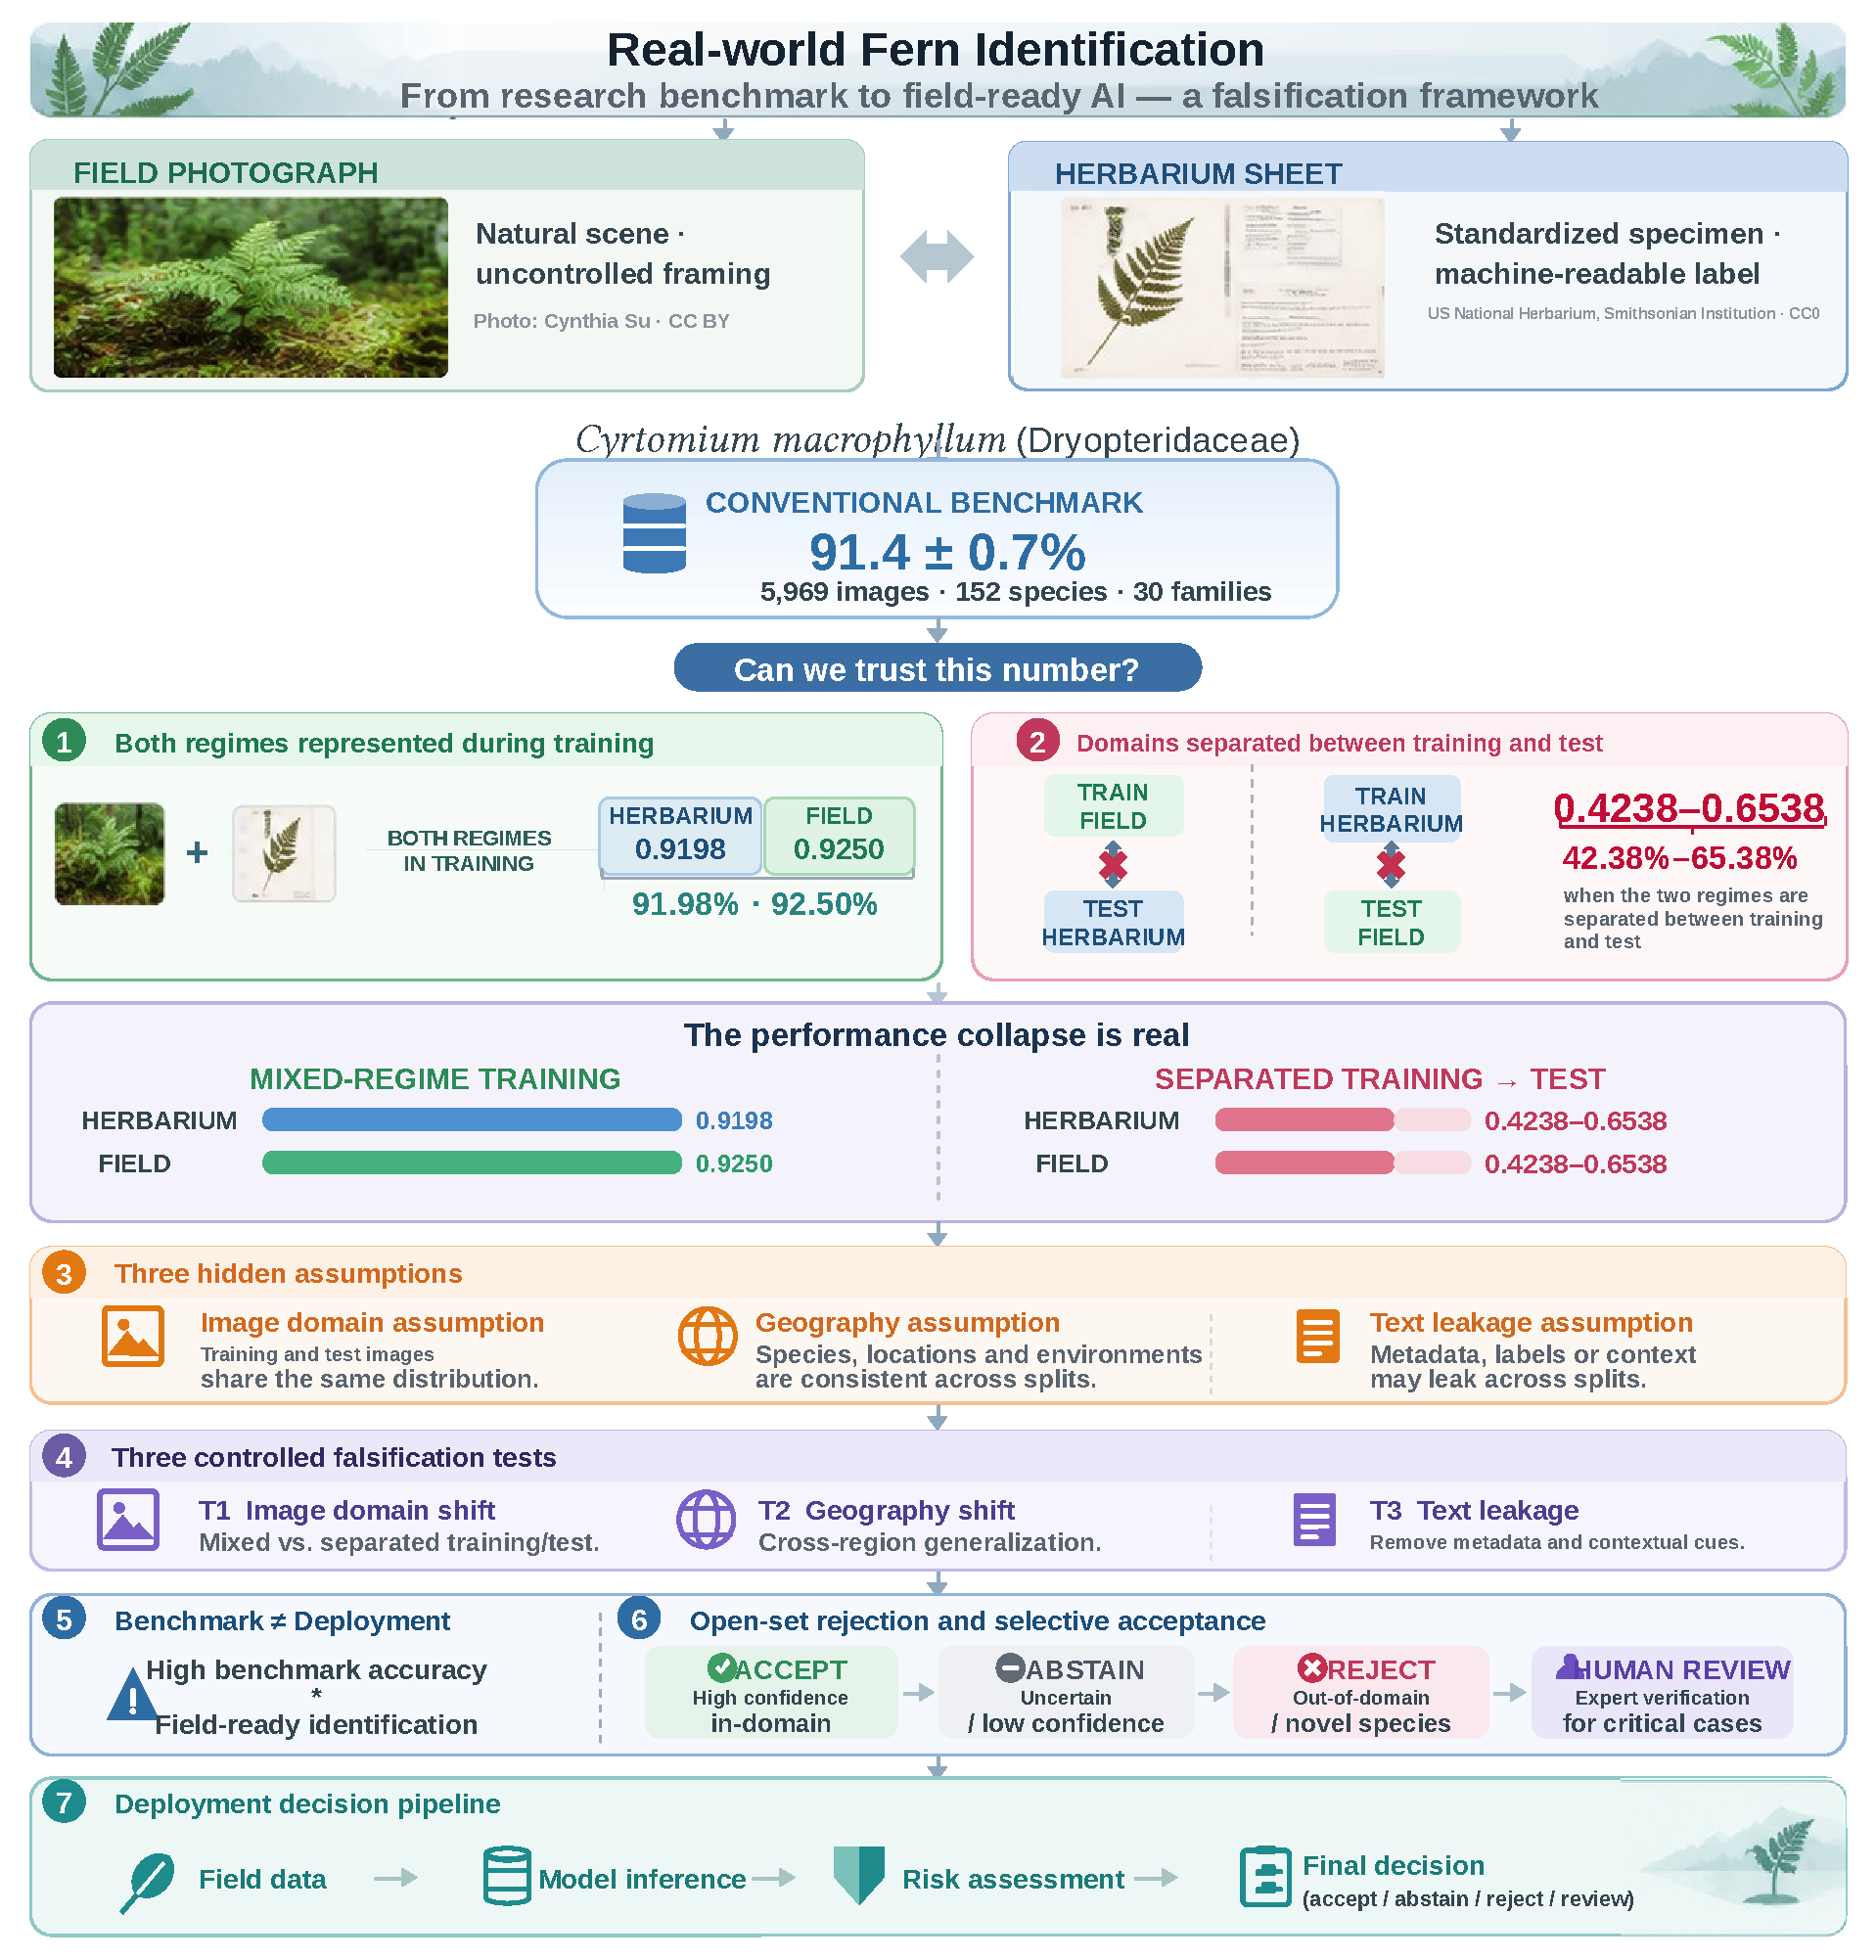
\includegraphics[width=\linewidth]{figures/Figure1_workflow.pdf}
\caption{From research benchmark to field-ready AI: a falsification framework for automated fern identification. The two image regimes of one species, \emph{Cyrtomium macrophyllum} (Dryopteridaceae), are field photographs (CC BY, Cynthia Su) and herbarium sheets (CC0, US National Herbarium, Smithsonian Institution). A conventionally split benchmark reports 91.4 $\pm$ 0.7\% over 5,969 images covering 152 species in 30 families. With both regimes represented during training the model reaches 0.9198 on sheets and 0.9250 on field photographs; separating the regimes between training and test drops accuracy to 0.4238--0.6538. Three hidden assumptions --- image domain, geography and text leakage --- are each tested by a controlled falsification test (T1--T3). Benchmark accuracy alone therefore does not make a model field-ready: the same model supports open-set rejection and selective acceptance, and a deployment decision pipeline routes field data through model inference and risk assessment to an accept, abstain, reject or review decision.}
\label{fig:1}
\end{figure}

The literature supplies evidence against each assumption, but never tests one in isolation. Studies of plant identification apps disagree --- high accuracy in a well-sampled European flora \citep{partel2021,rzanny2024} against unreliability on toxic and edible species \citep{long2023} and sensitivity to framing and scorers \citep{campbell2023,hart2023} --- and the disagreement is hard to settle because images and protocol differ at once. Occurrence records are strongly biased in space and taxonomy \citep{meyer2016}, and supplying geographic priors measurably changes fine-grained classification \citep{macaodha2019}, yet geographic holdout is rarely used as an evaluation axis: the community's benchmark varies acquisition mode instead \citep{martellucci2025}, and data scarcity itself has become the subject of a benchmark \citep{saputra2026}. Reviews of herbarium analysis treat label text and open-set conditions as unsettled \citep{geng2020,guo2025}, and testing the text assumption requires reading labels with an instrument other than the model under test.

Producing the measurement is unattractive for practical rather than conceptual reasons: it calls for a nested design in which each axis is compared against a baseline from the same subset of images, for labelled negatives and per-image confidence, which botanical benchmarks do not normally carry, and for a data requirement few taxa satisfy --- images in quantity in both visual regimes, per-image provenance, and licences permitting redistribution. Ferns meet the requirement only because digitised specimen records and volunteer observations are exposed through the same occurrence infrastructure \citep{gbifsecretariat2023}, and even then most of the resulting images cannot be redistributed \citep{scheffers2012}. Each piece is cheap in isolation; the combination is what has kept the question open.

We therefore ask four questions, which also determine the structure of the analysis that follows.

RQ1. Which pretraining source, adaptation mode, input resolution and output head give the best species-level identification on this benchmark, and does the ranking survive seed variance?

RQ2. How large are the accuracy losses when image domain, data source or geographic region are withheld, measured against baselines computed on the same images?

RQ3. How do a specialist identification API and two general-purpose vision--language models perform on the same images, and how much of their apparent accuracy on herbarium material depends on readable label text?

RQ4. Can the model's own confidence be used to automate decisions, in the sense of open-set rejection of non-fern images and selective prediction at controlled coverage?

Three of these close the assumptions above: RQ2 tests the first and second, RQ3 tests the third, and RQ1 establishes the instrument that makes all of them measurable. RQ4 asks a question the assumptions do not cover, because a monitoring workflow needs a decision rather than a label. We therefore treat the evaluation protocol, rather than the model, as the object of study, and use ferns to make it concrete: the benchmark assembles per-image annotations of image domain, source and country, splits by observation so that no occurrence straddles two splits, and pairs the positives with labelled fern-like negatives. Holding the model family fixed, we compare a frozen trunk against full fine-tuning, two input resolutions and a hierarchical head; the resulting recipe is statistically indistinguishable from fine-tuning across three seeds while training only a linear head, and we use it as a controlled instrument to test each assumption in turn. For RQ4, rejection is scored as a risk-coverage problem \citep{geifman2017} and calibration with the expected calibration error \citep{guo2017}.

We summarise our contributions as follows.

(i) A fern identification benchmark of 5,969 images covering 152 species in 30 families, with per-image annotations of image domain, data source and country, split by observation into 4,185 training, 882 validation and 902 test images, and accompanied by 700 open-set negatives in eight groups (Section~\ref{sec:3}).

(ii) A controlled comparison of recipe choices, in which biology-pretrained features with a frozen trunk and a linear head at 336 px perform best at 91.4 $\pm$ 0.7\% over three seeds, statistically indistinguishable from full fine-tuning and ahead of a general-purpose self-supervised backbone (RQ1; Section~\ref{sec:4}).

(iii) A test of the image-domain and geographic assumptions: crossing image domain or data source costs 8.6 to 48.1 percentage points, and holding out a region costs 3.6 to 39.8 percentage points, with the largest losses where species have the least out-of-region training support (RQ2; Sections~\ref{sec:5} and~\ref{sec:6}).

(iv) A test of the text-availability assumption, and an audit of general-purpose vision--language models and a specialist API on the same images: closed-set accuracy is 24 to 32\%, and open-ended accuracy after removing machine-readable names falls to 8.3 to 10.9\% (RQ3; Sections~\ref{sec:7} and~\ref{sec:8}).

(v) A deployment-oriented reading, in which the specialist model's confidence is conservative enough that accepting only the most confident quarter of images yields 100\% accuracy, whereas the API's confidence is not (RQ4; Sections~\ref{sec:9} and~\ref{sec:10}). Section~\ref{sec:11} returns to the question with which this paper opened.

---

\setcounter{section}{2}

\section{Construction Pipeline}\label{sec:3}

The benchmark is not a convenience sample. Three properties had to hold at once: both visual regimes of fern imagery are represented in quantity, every image carries enough provenance to define a distribution shift, and no individual plant can appear on both sides of an evaluation. Figure~\ref{fig:2} shows the pipeline; Table~\ref{tab:1} summarises its output.

\begin{table}[tbp]
\centering
\begin{threeparttable}
\caption{Composition of the fern benchmark}
\label{tab:1}
\begin{tabularx}{\linewidth}{>{\raggedright\arraybackslash\hsize=1.0\hsize}X >{\raggedright\arraybackslash\hsize=1.0\hsize}X >{\raggedright\arraybackslash\hsize=1.0\hsize}X}
\toprule
Item & Value & Note \\
\midrule
Images collected (full manifest) & 6,237 & dataset/manifest\_full.csv \\
Balanced working set ($\leq$60 images/species) & 5,969 & 268 over-cap images dropped; manifest\_balanced.csv \\
--- train / val / test & 4,185 / 882 / 902 & stratified by species, grouped by observation \\
Species / families & 152 / 30 & PPG I accepted names \\
Source: iNaturalist / GBIF & 3,157 / 2,812 & GBIF rows include iDigBio-digitised herbarium sheets \\
Image domain: field / specimen & 4,300 / 1,669 & specimen share 28.0\% \\
Countries (country\_clean, ISO-2) & 80 & UNK 330 rows (5.5\%) \\
Top countries & TW 1,886, CN 1,260, JP 391, UNK 330, US 316, RU 277 & full list in country\_distribution.csv \\
Open-set negatives & 700 & 8 groups (horsetail, lycophyte, moss, cycad, palm, angiosperm $\times$3, fungi, conifer) \\
Licence: redistributable / restricted & 1,432 / 4,537 & 1,432 images (24\%) cleared for public redistribution (release\_manifest.csv) \\
\bottomrule
\end{tabularx}

\end{threeparttable}
\end{table}

\begin{figure}[tbp]
\centering
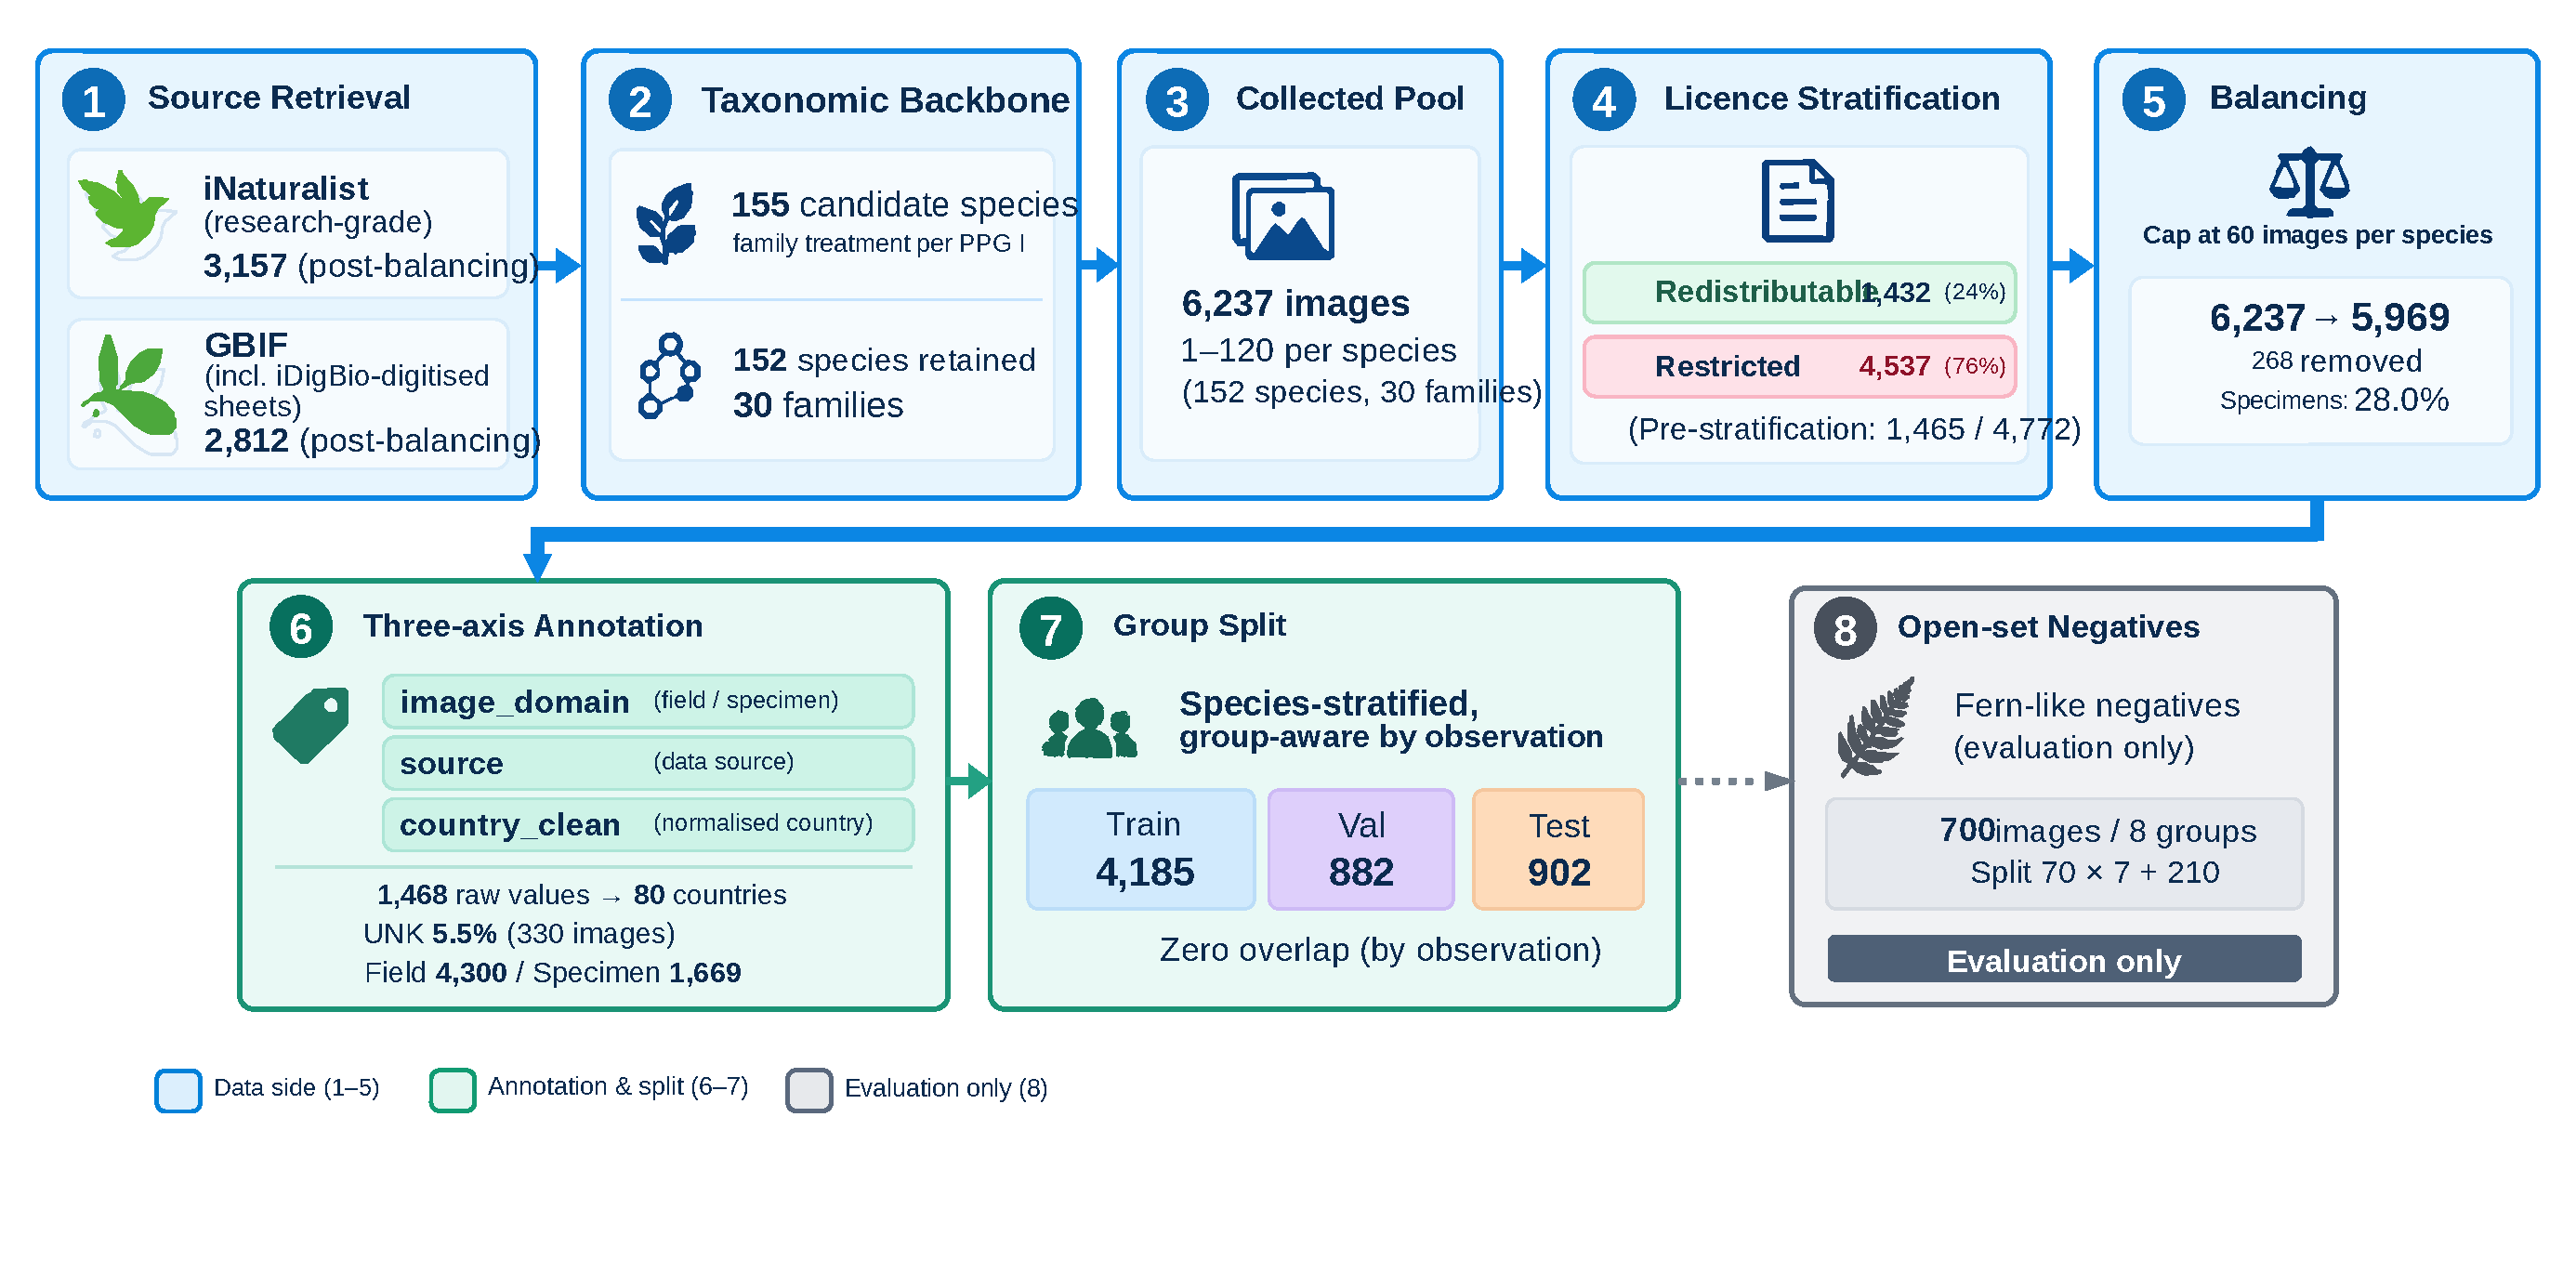
\includegraphics[width=\linewidth]{figures/Figure2_pipeline.pdf}
\caption{Benchmark construction. Records were retrieved from iNaturalist research-grade observations and from GBIF, including iDigBio-digitised herbarium sheets. The collected pool of 6,237 images was classified by licence, capped at 60 images per species and reduced to a working set of 5,969 images covering 152 species in 30 families, annotated with image domain, data source and normalised country, and split by observation into 4,185 training, 882 validation and 902 test images. A separate set of 700 fern-like negatives is used for evaluation only and never enters training.}
\label{fig:2}
\end{figure}

\setcounter{section}{3}

\setcounter{subsection}{0}

\subsection{Sources and queries}\label{sec:3.1}

Candidate taxa were taken from a reference atlas of Chinese higher plants (ferns, volumes 1--2), which supplied 155 species with Chinese and Latin names; the family treatment follows PPG I (2016). Occurrence records were then retrieved from two public sources, chosen because they carry different kinds of evidence rather than different amounts of it.

iNaturalist supplied research-grade observations, that is, records at least two identifiers have agreed on: photographs of living plants, taken opportunistically in the field. GBIF \citep{gbifsecretariat2023} supplied museum and aggregate records, a large fraction digitised herbarium sheets. The two sources differ not only in who made the image but in the physical object photographed, which is what makes them useful here.

Records were retained only when the occurrence matched one of the candidate species and the image was retrievable: 6,237 images covering 152 of the 155 candidate species in 30 families, with 1--120 images per species; three candidate species yielded no usable records and were dropped.

\setcounter{section}{3}

\setcounter{subsection}{1}

\subsection{Licence layering and the redistribution split}\label{sec:3.2}

Redistribution, not access, was the binding constraint. Each record was classified by its licence into redistributable (CC0, public domain, CC-BY, CC-BY-SA) or restricted (the non-commercial variants and everything else). Before balancing, 1,465 of the 6,237 images were redistributable, or 23\%; because the cap described below prefers openly licensed images when it has a choice, the share rises slightly in the working set, to 1,432 of 5,969 images, or 24\%. The remaining 4,537 images may be used for research and reported on, but cannot be republished by us. This asymmetry is stated here because it determines what the paper can hand to a reader; its consequences are set out in Section~\ref{sec:12}, and it is a general property of benchmark work built on citizen-science and museum records rather than a peculiarity of ferns.

\setcounter{section}{3}

\setcounter{subsection}{2}

\subsection{Balancing the working set}\label{sec:3.3}

The collected pool was strongly imbalanced, with a long tail of species represented by a handful of images and a few species by more than a hundred. Following common practice in fine-grained recognition benchmarks \citep{vanhorn2018}, the pool was capped at 60 images per species, which removed 268 over-cap images and left 5,969 images, between 1 and 60 per species. The working set contains 4,300 field photographs and 1,669 herbarium sheets, so specimens make up 28.0\% of it. Two details of the cap matter for later results: images were drawn round-robin across the two image domains, so capping does not silently collapse the domain balance (specimen share 27.8\% before, 28.0\% after), and preferentially retaining openly licensed images raises the redistributable share from 23\% to 24\%.

\setcounter{section}{3}

\setcounter{subsection}{3}

\subsection{Annotation axes}\label{sec:3.4}

Three provenance axes were recorded for every image, and they are what make the shifts in Sections~\ref{sec:5} and~\ref{sec:6} measurable rather than anecdotal.

\textbf{Image domain.} Each image was assigned to \texttt{field} or \texttt{specimen} from the machine-readable \texttt{basisOfRecord} field of the source record, not by manual inspection: preserved, living and material-sample records map to \texttt{specimen}, human and machine observations to \texttt{field}. Deriving the axis this way keeps the herbarium-versus-field contrast reproducible and independent of our own judgement.

\textbf{Data source.} Each image retains its originating platform, iNaturalist or GBIF, which after balancing contributes 3,157 and 2,812 images respectively.

\textbf{Country.} The country field of the source records is free text, mixing ISO-2 codes, iNaturalist place strings, Chinese addresses, Russian locality names and English-language addresses --- 1,468 distinct values in the training split alone. A normalisation step maps these to ISO-2 codes using ordered rules; everything unrecognised becomes \texttt{UNK}. The benchmark carries 80 countries plus 330 images with unknown country (5.5\%), and the raw values are retained alongside the normalised column so the mapping can be audited.

\setcounter{section}{3}

\setcounter{subsection}{4}

\subsection{Group-aware splits and evaluation subsets}\label{sec:3.5}

Images were split into training, validation and test sets stratified by species, and \emph{group-aware}: images sharing an observation or occurrence group are kept together, so a photographed individual, a duplicate sheet of the same gathering, or a set of frames from one observation never straddles two splits, which prevents a model from being credited for recognising an individual it saw during training.

The result is 4,185 training, 882 validation and 902 test images, covering 152, 150 and 150 species respectively; the intersection of the three splits is empty at the level of image identifier, file hash and group key. The two species that appear in the training split alone are those with the fewest images overall, discussed in Section~\ref{sec:8}.

Seven evaluation subsets are defined over the test split without moving or removing any image: by provenance, field only (640 images), specimen only (262), iNaturalist only (476) and GBIF only (426); by species frequency, 870 images for species with at least 30 balanced images and 32 for the rest. Sections~\ref{sec:5} and~\ref{sec:6} use these subsets to isolate each shift axis.

\setcounter{section}{3}

\setcounter{subsection}{5}

\subsection{Fern-like negatives}\label{sec:3.6}

A closed-set benchmark cannot evaluate rejection, and a deployment pipeline will encounter images that are not ferns at all. We therefore collected 700 additional images that a fern identifier should refuse to classify, drawn from the same sources and carrying the same manifest fields as the positives, so one pipeline can read both; they are used for evaluation only and never enter training.

The negatives are organised into eight groups, each defined by a taxon lookup rather than by hand-labelling, which keeps the group label auditable: three bracket the target taxa (horsetails \emph{Equisetum}, lycopods outside the benchmark's 155 species \emph{Selaginella}, and liverworts and mosses Marchantiophyta); two are the visually hardest case, plants whose fronds converge on fern morphology but which are not ferns (cycads \emph{Cycas} and palms Arecaceae); one is ordinary flowering plants (\emph{Rosa}, \emph{Trifolium}, \emph{Plantago}), which serves as an easy floor; and two cover taxa photographed in the same habitats (Agaricales fungi, \emph{Pinaceae} conifers). Group sizes are 70 each, except the flowering-plant group, which has 210 across its three genera. All negatives are research-grade records, normalised to RGB JPEG with a short side of at least 240 px, de-duplicated by SHA-1 hash, and released with unique identifiers. Section~\ref{sec:9} reports rejection performance on this set; per-group rates accompany the aggregate, which should not be read as an estimate for a deployment population.

\setcounter{section}{3}

\section{Model and Recipe}\label{sec:4}

The results follow the four research questions set out in Section~\ref{sec:2}, in the order in which they were posed. RQ1 comes first because it establishes the recipe that makes the remaining measurements comparable; RQ2 then tests the image-domain and geographic assumptions (Sections~\ref{sec:5} and~\ref{sec:6}); RQ3 audits the external systems and the text-availability assumption (Sections~\ref{sec:7} and~\ref{sec:8}); and RQ4 asks whether the model's own confidence can automate decisions (Section~\ref{sec:9}). Sections~\ref{sec:5} and~\ref{sec:6} attribute accuracy losses to the distribution of the data rather than to the model, and that attribution is only meaningful if the model is held fixed and reasonably well chosen. This section establishes the recipe used throughout, and reports how much of its ranking survives seed variance. Each section restates the question it answers; the interpretation of the measurements is taken up in Section~\ref{sec:10}.

\setcounter{section}{4}

\setcounter{subsection}{0}

\subsection{Backbones and adaptation modes}\label{sec:4.1}

Two pretrained visual backbones were compared under an identical protocol. BioCLIP 2 provides features pretrained on biological image--text data \citep{gu2025}; DINOv2 provides features pretrained by self-supervision on general imagery \citep{oquab2024}; the two are matched in architecture class, parameter count and input pipeline, so a difference between them is attributable to pretraining data. Two adaptation modes were used: in \texttt{linear} mode the trunk is frozen and only a LayerNorm projection and a linear classifier are trained; in \texttt{finetune} mode all parameters are updated. Both were evaluated because the literature does not settle which is preferable for fine-grained botanical tasks, and the answer sets the cost of redeploying the benchmark for a new taxon.

\setcounter{section}{4}

\setcounter{subsection}{1}

\subsection{Training protocol}\label{sec:4.2}

Input images were resized to 224 or 336 px. All runs used AdamW with weight decay 0.05, one warm-up epoch followed by cosine decay, label smoothing 0.1, gradient clipping at 1.0, mixed-precision arithmetic, and model selection on validation top-1 accuracy. Frozen-probe runs used 15 epochs, batch size 32 and a learning rate of 1e-3, except at 224 px, where the batch size was 64. The 336 px fine-tuned run used 12 epochs, batch size 16 and a learning rate of 2e-5. The reference seed is 20261010, and two further seeds were run for the key configurations. Every run saw the same 4,185 training and 902 test images, with 152 output classes.

\setcounter{section}{4}

\setcounter{subsection}{2}

\subsection{Recipe comparison}\label{sec:4.3}

Table~\ref{tab:2} and Figure~\ref{fig:3} report eleven configurations. The best recipe is a frozen BioCLIP 2 trunk with a linear head at 336 px. It scores 0.9235 in its best seed, or 0.9139 $\pm$ 0.0073 over three seeds (91.4 $\pm$ 0.7\%). The same backbone at 224 px reaches 0.8980, so resolution is worth 2.5 pp (paired McNemar p = 0.005, single seed). Zero-shot BioCLIP 2, with no training at all, already reaches 0.6829 at species level, 0.8381 within the top three, and 0.290 at family level. Replacing biological pretraining with general self-supervision costs more than any other single change. DINOv2 reaches 0.8433 $\pm$ 0.0050 at 336 px. BioCLIP 2 is therefore ahead by +7.1 $\pm$ 1.0 pp in a paired comparison across three seeds, and the ordering is the same at 224 px.

\begin{table}[tbp]
\centering
\caption{Main results on the 902-image test split}
\label{tab:2}
\resizebox{\linewidth}{!}{%
\begin{tabular}{llllllllll}
\toprule
Configuration & Mode & px & train\_n & test\_n & Species top-1 & top-3 & macro & specimen & field \\
\midrule
BioCLIP 2 / frozen / 336 & linear & 336 & 4185 & 902 & 0.9235 & 0.9778 & 0.9227 & 0.9198 & 0.9250 \\
BioCLIP 2 / fine-tuned / 336 & finetune & 336 & 4185 & 902 & 0.9013 & 0.9723 & 0.8957 & 0.9122 & 0.8969 \\
BioCLIP 2 / frozen / 224 & linear & 224 & 4185 & 902 & 0.8980 & 0.9767 & 0.8952 & 0.8969 & 0.8984 \\
BioCLIP 2 / frozen / 224 + class-bal. & linear & 224 & 4185 & 902 & 0.8980 & 0.9690 & 0.8956 & 0.8893 & 0.9016 \\
BioCLIP 2 / fine-tuned / 224 & finetune & 224 & 4185 & 902 & 0.8914 & 0.9690 & 0.8905 & 0.9046 & 0.8859 \\
BioCLIP 2 / fine-tuned / 224 (lr 5e-5) & finetune & 224 & 4185 & 902 & 0.8459 & 0.9534 & 0.8424 & 0.8855 & 0.8297 \\
BioCLIP 2 / fine-tuned / 224 + hier. head & finetune & 224 & 4185 & 902 & 0.8614 & 0.9612 & 0.8504 & 0.8779 & 0.8547 \\
DINOv2 / fine-tuned / 224 & finetune & 224 & 4185 & 902 & 0.8592 & 0.9512 & 0.8516 & 0.8702 & 0.8547 \\
DINOv2 / frozen / 336 & linear & 336 & 4185 & 902 & 0.8437 & 0.9412 & 0.8346 & 0.8626 & 0.8359 \\
DINOv2 / frozen / 224 & linear & 224 & 4185 & 902 & 0.7927 & 0.9357 & 0.7760 & 0.8015 & 0.7891 \\
BioCLIP 2 / zero-shot (no training) & zero-shot & 224 & 0 & 902 & 0.6829 & 0.8381 & 0.6864 & 0.6069 & 0.7141 \\
BioCLIP 2 / frozen / 336 --- seed mean$\pm$sd & linear & 336 & 4185 & 902 & 0.9139 $\pm$ 0.0073 & --- & --- & --- & --- \\
BioCLIP 2 / fine-tuned / 336 --- seed mean$\pm$sd & finetune & 336 & 4185 & 902 & 0.9084 $\pm$ 0.0041 & --- & --- & --- & --- \\
DINOv2 / frozen / 336 --- seed mean$\pm$sd & linear & 336 & 4185 & 902 & 0.8433 $\pm$ 0.0050 & --- & --- & --- & --- \\
\bottomrule
\end{tabular}
}
\par\vspace{3pt}
\noindent\begin{minipage}{\linewidth}\footnotesize
Note. Rows are single-seed (20261010) unless marked; the last three rows give the mean $\pm$ sd (population sd, ddof=0) over three seeds (20261010/11/12).
\end{minipage}
\end{table}

\begin{figure}[tbp]
\centering
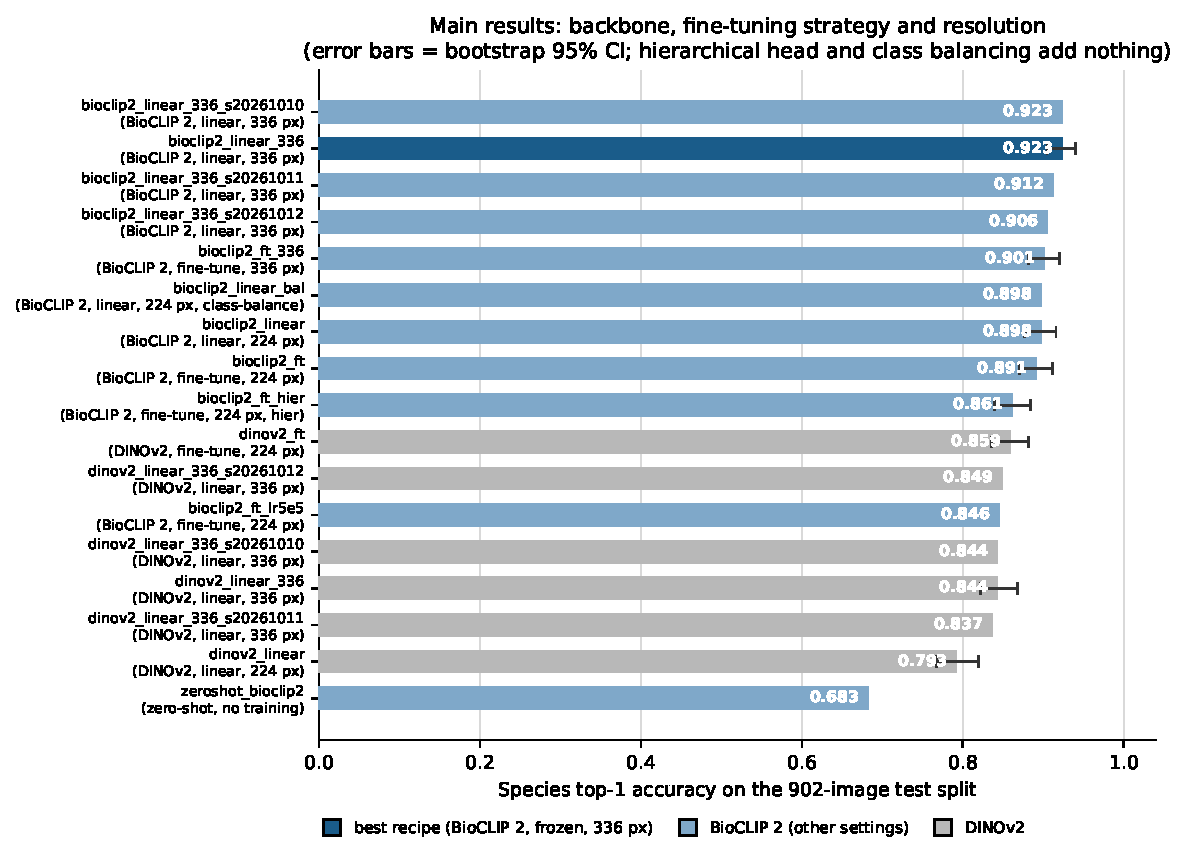
\includegraphics[width=\linewidth]{figures/Figure3_main_results.pdf}
\caption{Species top-1 accuracy on the 902-image test split for eleven configurations of backbone, adaptation mode, input resolution and head design, with the frozen linear probe at 336 px shown first. The hierarchical head is the only configuration below the general-purpose self-supervised backbone. Error bars are the standard deviation over three seeds where available; single-seed configurations are marked.}
\label{fig:3}
\end{figure}

Two recipe choices did not help, and both are reported rather than omitted: a hierarchical head with a family-level auxiliary loss produced 0.8614, 6.0 pp below the main recipe (paired McNemar p \textless{} 1e-16), though that configuration also differs in resolution and learning rate, so the difference is not a clean estimate of what a hierarchical head costs; and class-balanced sampling changed macro-averaged accuracy by 0.04 pp.

\setcounter{section}{4}

\setcounter{subsection}{3}

\subsection{Seed variance and the frozen-versus-fine-tuned question}\label{sec:4.4}

The fine-tuned 336 px configuration is the only variant close enough to the main recipe to need a careful comparison, and seed variance decides it. Across three seeds it reaches 0.9084 $\pm$ 0.0041, against 0.9139 $\pm$ 0.0073 for the frozen probe. Pairing by seed gives differences of +2.00, +0.44 and $-$0.78 pp, a mean of +0.55 $\pm$ 1.13 pp whose interval includes zero; in one seed the fine-tuned model is ahead. A single-seed paired test would have reported p = 0.025 in favour of the frozen probe, and that value does not survive the seed-level comparison, so it is not used as evidence here. The frozen probe is used for every result that follows, because it trains only a linear head, and its seed-to-seed standard deviation of 0.7 pp is smaller than the smallest shift effect reported later (3.6 pp), so the shifts that follow are not seed noise.

\setcounter{section}{4}

\setcounter{subsection}{4}

\subsection{Reproducibility}\label{sec:4.5}

Training is deterministic for the frozen-probe configuration: rerunning the reference seed reproduces its accuracy exactly. The fine-tuned configuration contains non-deterministic CUDA kernels (about $\pm$0.22 pp per re-run), which three-seed means cover; where a comparison could not be repeated across seeds, the tables label it as a single-seed result.

\setcounter{section}{4}

\section{Domain and Source Shift}\label{sec:5}

The first assumption built into a mixed benchmark is that a herbarium sheet and a field photograph of the same species are interchangeable evidence. This section tests it by training on one image regime or source and testing on another, and by comparing each result against a baseline computed on the same images.

\setcounter{section}{5}

\setcounter{subsection}{0}

\subsection{Transfer protocol and the subset-matched baseline}\label{sec:5.1}

Four directions were run, each with the recipe fixed as in Section~\ref{sec:4} and trained on the full training split restricted to one regime or source. The label space was rebuilt from the filtered training split, so the number of classes differs by direction: 90 for GBIF-trained models, 122 for iNaturalist-trained, 71 for specimen-trained and 137 for field-trained. Test sets were likewise restricted, and further restricted to species the model had seen during training, giving 128, 270, 156 and 210 images respectively.

A transfer result means nothing without a matched reference, because a class-restricted test subset is intrinsically harder than the full test split. The baseline used here is the full model of Section~\ref{sec:4} scored on the identical subset of images --- the same convention as the geographic holdouts of Section~\ref{sec:6}. Using the mixed-set accuracy instead would conflate the cost of the shift with the difficulty of the subset, and would overstate every drop.

One caveat belongs here. The transfer runs did not emit per-image predictions, so their baselines were recomputed from the main model's per-image records over reconstructed subsets; the reconstruction reproduces the exact test-set sizes recorded for each run, but on the smallest subset (128 images) a single image is worth 0.8 pp, and differences below about 1 pp should not be read as effects.

\setcounter{section}{5}

\setcounter{subsection}{1}

\subsection{Cross-domain and cross-source results}\label{sec:5.2}

Table~\ref{tab:3} and Figure~\ref{fig:4} report the four directions. All four lose accuracy, and the losses span an order of magnitude.

\begin{table}[tbp]
\centering
\caption{Domain / source transfer under the corrected protocol}
\label{tab:3}
\resizebox{\linewidth}{!}{%
\begin{tabular}{lllllllllll}
\toprule
Experiment & Train on & Test on & Classes & train\_n & test\_n & top-1 & macro & in-domain (same subset) & $\Delta$ (pp) & previous value \\
\midrule
Cross-source & GBIF & iNaturalist & 90 & 1965 & 128 & 0.7891 & 0.8071 & 0.8750 & -8.6 & 0.2059 (defective) \\
Cross-domain & specimen & field & 71 & 1166 & 156 & 0.6538 & 0.7260 & 0.8526 & -19.9 & 0.3244 (defective) \\
Cross-source & iNaturalist & GBIF & 122 & 2220 & 270 & 0.5000 & 0.5697 & 0.9000 & -40.0 & 0.3239 (defective) \\
Cross-domain & field & specimen & 137 & 3019 & 210 & 0.4238 & 0.4285 & 0.9048 & -48.1 & 0.1500 (defective) \\
In-domain & all & all & 152 & 4185 & 902 & 0.9235 & 0.9227 & 0.9235 & 0.0 & --- \\
\bottomrule
\end{tabular}
}
\par\vspace{3pt}
\noindent\begin{minipage}{\linewidth}\footnotesize
Note. The label space is rebuilt from the filtered training split. 'in-domain (same subset)' is the same full model scored on the identical test subset (the convention already used in Table~\ref{tab:4}), so $\Delta$ = top-1 $-$ in-domain isolates the transfer cost from subset composition. The last column keeps the values published before the label-space correction.
\end{minipage}
\end{table}

\begin{figure}[tbp]
\centering
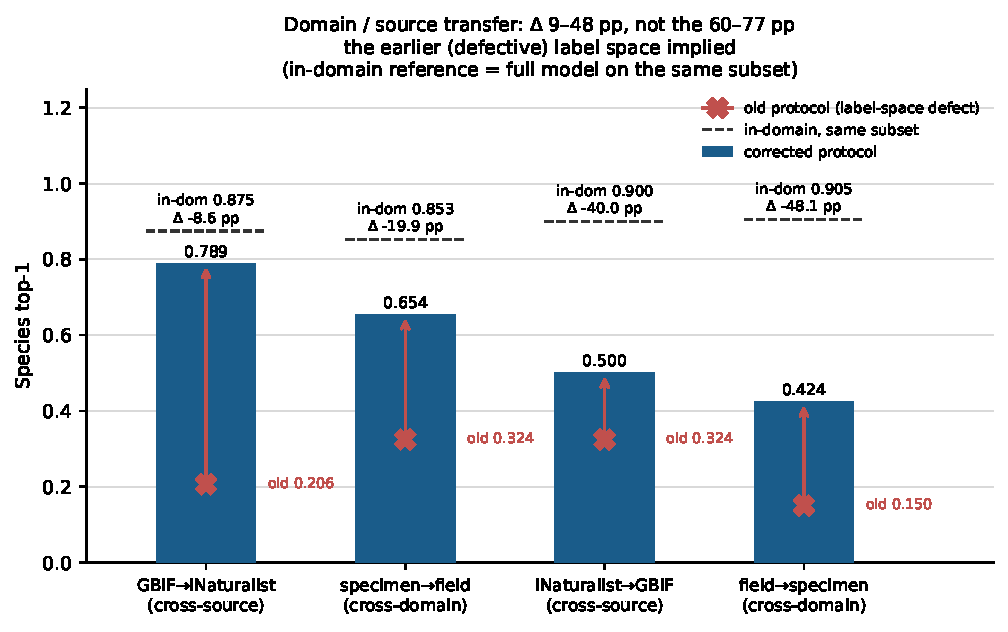
\includegraphics[width=\linewidth]{figures/Figure4_transfer_drops.pdf}
\caption{Cost of transferring across image domain or data source, each measured against an in-domain baseline computed on the identical subset of test images, so the difference isolates the effect of the split rather than the difficulty of the subset. Crosses mark the values published under the earlier label-space protocol, which are superseded.}
\label{fig:4}
\end{figure}

Training on digitised specimens and testing on field photographs costs $-$19.9 pp (0.6538 against an in-domain 0.8526). The reverse direction is the most damaging single result in the paper: training on field photographs and testing on specimens costs $-$48.1 pp (0.4238 against 0.9048).

The two source crossings behave similarly but less symmetrically: GBIF-trained to iNaturalist costs $-$8.6 pp (0.7891 against 0.8750), and the reverse costs $-$40.0 pp (0.5000 against 0.9000). Source and image domain are correlated, since most GBIF records in this corpus are sheets and most iNaturalist records are field photographs, so these two axes are not fully independent. Section~\ref{sec:6} addresses the geographic axis, which is independent of both by construction.

\setcounter{section}{5}

\setcounter{subsection}{2}

\subsection{Where the iNaturalist-to-GBIF cost comes from}\label{sec:5.3}

The iNaturalist-to-GBIF direction can be decomposed because the GBIF test images carry both source and image-domain labels. Within that 270-image test set, the model scores 0.741 on the field photographs and 0.340 on the herbarium sheets. The cost is therefore not spread evenly across the source: it is concentrated in the sheet subpopulation.

\setcounter{section}{5}

\setcounter{subsection}{3}

\subsection{Protocol correction}\label{sec:5.4}

The transfer results reported here do not agree with an earlier run of the same experiments, and the reason matters for interpreting any transfer number.

In the original implementation the label space was taken from the unfiltered training split, so species removed by the domain or source filter retained their class indices and competed for every test image with randomly initialised weights --- in the field-to-specimen direction, 81 of the 152 output classes were spurious. The effect was systematic rather than random: a class-restricted model had fewer real classes, a larger share of the output space was noise, and the collapse appeared far more severe than it is. Rebuilding the label space from the filtered split removes the defect, changing the four transfer accuracies from 0.2059, 0.3239, 0.3244 and 0.1500 to the values in Table~\ref{tab:3}.

Figure~\ref{fig:4} retains the superseded values as separate markers, and a before-and-after comparison is given in the Supplementary Material.

\setcounter{section}{5}

\section{Geographic Shift}\label{sec:6}

The second assumption is that geographic provenance is exchangeable: that a species' test images arise under the same conditions as its training images, so that recognising a species is equivalent to recognising it anywhere. This section tests that assumption directly by removing a region from training and evaluating on it.

\setcounter{section}{6}

\setcounter{subsection}{0}

\subsection{Leave-one-region-out protocol}\label{sec:6.1}

Eight holdouts were run. For each, the model was trained on the whole training split except images from the held-out region. Both the validation and test sets were then restricted to that region and, as in Section~\ref{sec:5}, to species the model had seen during training. The recipe is the one fixed in Section~\ref{sec:4}, at 336 px and 15 epochs.

Two properties make the result interpretable: the comparison column is the same full model scored on the identical test subset, so the difference is the effect of having seen the region rather than a difference between models; and the held-out regions are not mutually exclusive --- the China-region row aggregates Mainland China with Taiwan, China, Hong Kong, China and Macao, China, and overlaps two other rows, so the eight values are eight measurements of one phenomenon, not eight independent countries.

The geographic annotation is derived, as described in Section~\ref{sec:3.4}. Of the 330 images whose country could not be established, 131 carry no location information at all and the remainder use formats the normaliser does not cover. All are excluded from the geographic analysis, so every number in this section rests on the remaining 5,639 images.

\setcounter{section}{6}

\setcounter{subsection}{1}

\subsection{Results across the holdouts}\label{sec:6.2}

Table~\ref{tab:4} and Figure~\ref{fig:5} report the results. Every holdout reduces accuracy, and the spread is wide: from $-$3.6 pp for Vietnam to $-$39.8 pp for Taiwan, China.

\begin{table}[tbp]
\centering
\caption{Leave-one-region-out geographic holdout}
\label{tab:4}
\resizebox{\linewidth}{!}{%
\begin{tabular}{llllllll}
\toprule
Held-out region & Classes & train\_n & test\_n & held-out model & in-domain & $\Delta$ (pp) & specimen share \\
\midrule
Taiwan, China & 145 & 2860 & 244 & 0.5615 & 0.9590 & -39.8 & 0.02 \\
Mainland China & 146 & 3293 & 171 & 0.6959 & 0.9006 & -20.5 & 0.58 \\
China region (incl. Taiwan, Hong Kong, Macao) & 130 & 1902 & 367 & 0.6158 & 0.9428 & -32.7 & 0.26 \\
Japan & 152 & 3901 & 59 & 0.7966 & 0.9492 & -15.3 & 0.34 \\
Thailand & 152 & 4029 & 31 & 0.6452 & 0.7742 & -12.9 & 0.81 \\
United States & 152 & 3963 & 47 & 0.9149 & 0.9787 & -6.4 & 0.00 \\
Russia & 152 & 4011 & 54 & 0.9259 & 0.9815 & -5.6 & 0.04 \\
Vietnam & 151 & 4088 & 28 & 0.8214 & 0.8571 & -3.6 & 0.75 \\
\bottomrule
\end{tabular}
}
\par\vspace{3pt}
\noindent\begin{minipage}{\linewidth}\footnotesize
Note. The in-domain column is the same full model scored on the identical test subset, so $\Delta$ = held-out $-$ in-domain isolates 'having seen the region'; negative values are performance lost by holding the region out.
\end{minipage}
\end{table}

\begin{figure}[tbp]
\centering
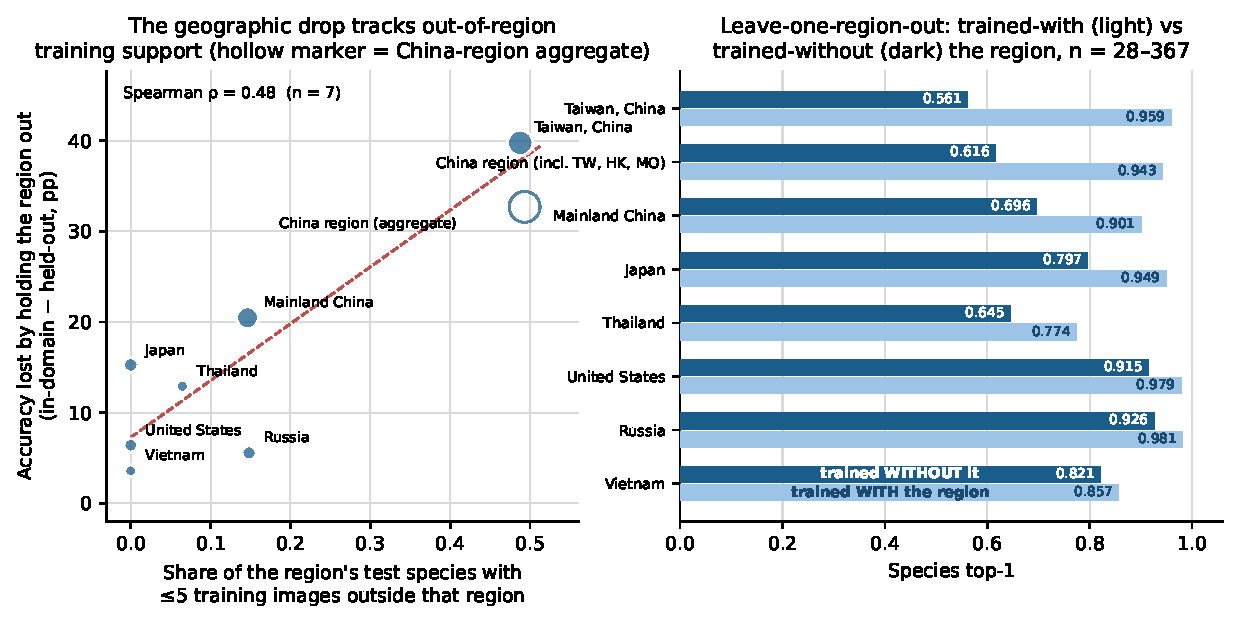
\includegraphics[width=\linewidth]{figures/Figure5_geographic_holdout.pdf}
\caption{Leave-one-region-out geographic holdout. (a) Accuracy of the holdout model against the in-domain model scored on the same test images. (b) Absolute accuracy for each held-out region. (c) The accuracy drop against the share of the region's test species with at most five training images from outside that region. The association is positive but weak, and the aggregate point for the China region is shown separately.}
\label{fig:5}
\end{figure}

The pattern separates the holdouts into two groups: Taiwan, China ($-$39.8, from 0.9590 to 0.5615) and the China region ($-$32.7) lose most; Mainland China ($-$20.5), Japan ($-$15.3) and Thailand ($-$12.9) lose moderately; the United States ($-$6.4), Russia ($-$5.6) and Vietnam ($-$3.6) lose little. Both groups are geographically Asian, so the separation is not between continents --- what distinguishes them is how much of each species' training support lies elsewhere, which is the subject of the next subsection.

\setcounter{section}{6}

\setcounter{subsection}{2}

\subsection{Association with out-of-region training support}\label{sec:6.3}

For each holdout we computed the share of its test images whose species has five or fewer training images outside the held-out region. This share ranges from 0.49 (Taiwan, China, and the China region) to 0.00 (Japan, the United States, Vietnam). It tracks the size of the drop. The two holdouts with the thinnest out-of-region support lose 39.8 and 32.7 pp; the three with complete support lose 15.3 pp or less.

Across the seven country-level holdouts the association is positive but weak: Spearman $\rho$ = 0.48 (n = 7, p $\approx$ 0.28). Including the China-region aggregate raises it to 0.63 (n = 8, p $\approx$ 0.09). Neither is significant at conventional levels. Figure~\ref{fig:5}C plots the eight points with the fitted trend.

Two deviations are visible in that plot and are worth stating rather than smoothing over. Russia has a thin-support share of 0.15 but loses only 5.6 pp, and Japan has complete support yet loses 15.3 pp; with 54 and 59 test images respectively, both are noisy estimates, but they show that out-of-region support is not the only term. The image-domain composition of each country's test set also differs, from 2\% specimens for Taiwan, China to 81\% for Thailand, and the domain axis carries its own cost of up to 48 pp (Section~\ref{sec:5}), so the holdout drops contain a domain component this analysis does not separate.

The hypothesis we started with is the one we cannot report: if geographic loss were driven by species unique to a region, holdouts covering more such species should lose more, but because the split is stratified by species no species is confined to a single country and every species occurs in at least two. The first explanation we tested was therefore refuted by the design of the benchmark itself.

What these results support operationally is taken up in Section~\ref{sec:10}.

\setcounter{section}{6}

\section{External Systems and the Text-Availability Assumption}\label{sec:7}

The third assumption is that a reported accuracy reflects morphological identification. That assumption is hardest to test on a specialist classifier and easiest to test on models that read text, and general-purpose vision--language models can do both. This section evaluates three external systems on the same 902 test images, then tests the assumption with an independent reading of the labels.

\setcounter{section}{7}

\setcounter{subsection}{0}

\subsection{A specialist identification API}\label{sec:7.1}

Pl@ntNet was queried through its public identification service, using the full referential --- the configuration a practitioner would use. It scores 0.2428 at species level (95\% CI 0.215--0.272), 0.312 within the top three, 0.506 at genus level and 0.367 at family level. For 64.9\% of test images the true species was not among its ten candidates; its species-level score is less than half its genus-level score.

Split by image domain, the failure is not uniform: 0.341 on field photographs against 0.004 on herbarium sheets --- one sheet out of 262 right. The split by source is equally uneven: 0.368 on iNaturalist images and 0.103 on GBIF images.

Two of the 902 images returned HTTP 404 from the service, and repeated attempts reproduced the failure; re-encoding and resizing did not help, and a same-sized control image passes, so the trigger is the image content. Scaling the long side to 1024 px makes both images succeed. The evaluation therefore includes a fallback path that downscales and retries, and marks the affected records rather than merging them silently.

\setcounter{section}{7}

\setcounter{subsection}{1}

\subsection{Two general-purpose vision--language models}\label{sec:7.2}

Two models from independent families were evaluated: Qwen3.7-flash through its commercial API, and Qwen3-VL-8B-Instruct served locally \citep{bai2025}. Table~\ref{tab:5} places both alongside the specialist systems on the same images. Each saw the same 902 test images twice: in the open-ended task it was asked to name the species with no candidate list; in the closed-set task it was given the 152 species names and asked to choose one, making it directly comparable to the classifier of Section~\ref{sec:4}.

\begin{table}[tbp]
\centering
\caption{All systems on the same 902-image test split}
\label{tab:5}
\resizebox{\linewidth}{!}{%
\begin{tabular}{lllllll}
\toprule
System & Task & n & Species top-1 & Species top-3 & Family top-1 & top-1, leakage removed \\
\midrule
BioCLIP 2, frozen + linear @336 (ours) & closed-set species & 902 & 0.9235 & 0.9778 & 0.971 \dag{} & --- \\
DINOv2, frozen + linear @336 & closed-set species & 902 & 0.8437 & 0.9412 & 0.932 \dag{} & --- \\
Pl@ntNet API (\texttt{all} referential) & open-ended & 902 & 0.2428 & 0.312 & 0.367 & --- \\
Qwen3.7-flash (DashScope API) & open-ended & 901 & 0.1587 & 0.1876 & 0.522 & 0.1092 \\
Qwen3-VL-8B (local vLLM) & open-ended & 902 & 0.1364 & 0.1663 & 0.480 & 0.0825 \\
Qwen3.7-flash (DashScope API) & closed-set species & 901 & 0.3196 & 0.4151 & --- & 0.2609 \\
Qwen3-VL-8B (local vLLM) & closed-set species & 902 & 0.2417 & 0.3060 & --- & 0.1833 \\
\bottomrule
\end{tabular}
}
\par\vspace{3pt}
\noindent\begin{minipage}{\linewidth}\footnotesize
Note. \dag{} Family accuracy derived from the species head (the VLMs instead saw an explicit 30-way family task). The last column removes images whose true name is OCR-readable on the sheet.
\end{minipage}
\end{table}

On the open-ended task the two models reach 0.1587 and 0.1364 at species level. On the closed-set task, where guessing has a 1-in-152 chance, they reach 0.3196 and 0.2417. Both are an order of magnitude below the specialist classifier's 0.9235 in the reference seed on the same images, and the paired differences are large and unambiguous: +60.3 pp against the better of the two on the closed-set task, and +80.8 to +83.5 pp against the open-ended runs once leaked images are removed (Section~\ref{sec:7.5}, Table~\ref{tab:6}).

\begin{table}[tbp]
\centering
\caption{Paired McNemar tests on the shared test images}
\label{tab:6}
\resizebox{\linewidth}{!}{%
\begin{tabular}{llllll}
\toprule
Comparison & n (paired) & $\Delta$ top-1 (pp) & McNemar p & sig. & 95\% CI of $\Delta$ \\
\midrule
bioclip2\_linear\_336 vs dinov2\_linear\_336 & 902 & +7.8 & 0.00e+00 & *** & [+5.5, +10.1] \\
bioclip2\_linear\_336 vs bioclip2\_ft\_336 & 902 & +2.1 & 2.48e-02 & * & [+0.4, +3.9] \\
bioclip2\_linear\_336 vs bioclip2\_ft\_hier & 902 & +6.0 & 0.00e+00 & *** & [+4.0, +8.1] \\
bioclip2\_linear\_336 vs bioclip2\_linear & 902 & +2.5 & 5.15e-03 & ** & [+0.9, +4.3] \\
bioclip2\_linear\_336 vs plantnet\_all & 902 & +68.0 & 0.00e+00 & *** & [+64.8, +71.1] \\
bioclip2\_linear\_336 vs qwen3.7-flash\_species152 & 901 & +60.3 & 0.00e+00 & *** & [+56.8, +63.6] \\
bioclip2\_linear\_336 vs qwen3-vl-8b\_species152 & 902 & +68.1 & 0.00e+00 & *** & [+64.9, +71.2] \\
bioclip2\_linear\_336 vs qwen3.7-flash\_open\_noleak & 824 & +80.8 & 0.00e+00 & *** & [+78.0, +83.5] \\
bioclip2\_linear\_336 vs qwen3-vl-8b\_open\_noleak & 824 & +83.5 & 0.00e+00 & *** & [+80.8, +86.0] \\
dinov2\_linear\_336 vs dinov2\_ft & 902 & -1.4 & 2.67e-01 & n.s. & [-3.8, +0.9] \\
plantnet\_all vs qwen3.7-flash\_open & 901 & +8.4 & 1.00e-05 & *** & [+4.8, +12.2] \\
\bottomrule
\end{tabular}
}
\par\vspace{3pt}
\noindent\begin{minipage}{\linewidth}\footnotesize
Note. All systems saw the same images; \textbf{* p\textless{}0.001, } p\textless{}0.01, * p\textless{}0.05, n.s. = not significant. Full 105-pair matrix in paired\_mcnemar\_v2.csv. \textbf{All tests are single-seed (20261010):} the bioclip2\_linear\_336 vs bioclip2\_ft\_336 row (+2.1 pp, p=0.025) does NOT survive seed variance -- across three seeds the paired difference is +2.00 / +0.44 / -0.78 pp (mean +0.55 $\pm$ 1.13 pp, interval includes zero), so frozen and fine-tuned are statistically indistinguishable. Cite the seed-level result (Table~\ref{tab:2} and RESULTS.md \S{}14), not this single-seed p-value.
\end{minipage}
\end{table}

The domain breakdown is what directed the rest of this section. Pl@ntNet failed on sheets and succeeded on field photographs; the language models did the opposite: Qwen3.7-flash reaches 0.069 on field photographs and 0.379 on herbarium sheets. The rest of this section tests the alternative explanation, that the models read the labels rather than identified the plants.

\setcounter{section}{7}

\setcounter{subsection}{2}

\subsection{Text-leakage audit with an independent OCR pass}\label{sec:7.3}

The assumption was tested with an instrument other than the models under test: every image was passed through an optical character recognition engine, and the recognised text was searched for the true species name. The two image domains separate cleanly: no field photograph yielded the species name as machine-readable text, and only 0.2\% carried more than 40 characters of text at all, while among herbarium sheets 0.298 yielded the species name directly and 0.847 carried at least 40 characters of printed label text. Across the whole test set the name was available as text for 8.6\% of images.

Accuracy follows that boundary: on the machine-readable subset Qwen3.7-flash reaches 0.688, while on the clean subset the same model reaches 0.250 on sheets and 0.069 on field photographs. The leaky subset is therefore three times easier than the clean one, and the advantage appears only where text exists. Removing every image whose species name is machine-readable gives the models' morphological accuracy as 0.1092 and 0.0825 on the open-ended task, and 0.2609 and 0.1833 on the closed-set task. The overall leakage rate of 8.6\% is a lower bound, because optical character recognition reads printed labels far better than handwritten ones and the models can read both, so 10.9\% is an upper bound rather than an estimate: the more leakage the audit missed, the lower the true morphological accuracy falls.

\setcounter{section}{7}

\setcounter{subsection}{3}

\subsection{Calibration and selective prediction}\label{sec:7.4}

A model whose confidence is trustworthy can be deployed with a rejection option; one whose confidence is not cannot. The two specialist systems differ in opposite directions. Our classifier is under-confident, with an expected calibration error of 0.195 over ten bins; its stated confidence sits below its observed accuracy in every bin, and its most confident bin is correct on every image in it. Pl@ntNet is systematically over-confident, with an expected calibration error of 0.090, and the gap widens as confidence rises: its most confident bin claims 0.943 and delivers 0.683. Thresholding Pl@ntNet's score at 0.5 raises its accuracy from 0.243 to 0.590 but covers only a quarter of the images, and 41\% of those it accepts are wrong.

Accepting the classifier's most confident 25\% of images gives 100\% accuracy, accepting the most confident half keeps accuracy above 0.99, and accepting 85\% still holds 0.967; Pl@ntNet's score supports no such policy. The full risk-coverage behaviour of both systems is shown in Figure~\ref{fig:7}, their reliability diagrams in Figure~\ref{fig:6}. Latency separates the systems by two orders of magnitude: the classifier runs at 22.6 ms per image on a single consumer-grade GPU, the external systems take 1.8 to 3.4 s. Full fine-tuning is the one configuration with a different calibration profile --- better calibrated than the frozen probe (expected calibration error 0.095 against 0.195) but less accurate (Section~\ref{sec:4}) --- so the frozen probe is the configuration reported above.

\begin{figure}[tbp]
\centering
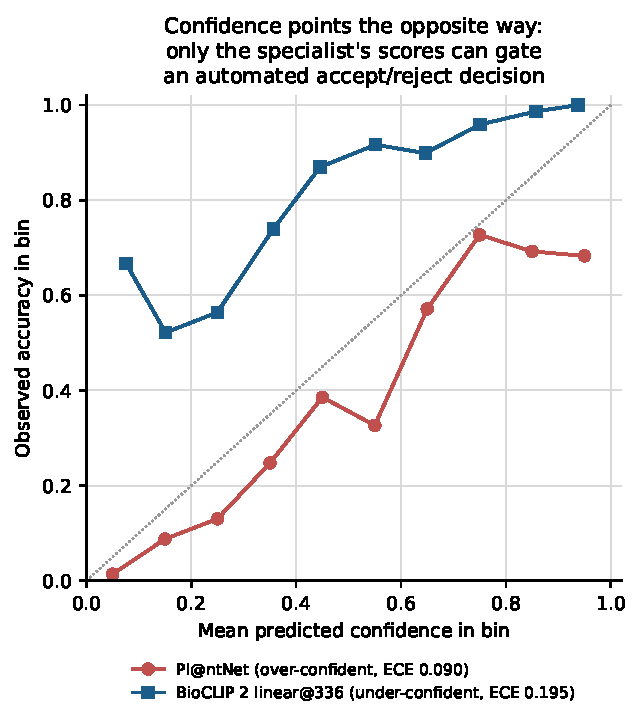
\includegraphics[width=\linewidth]{figures/Figure6_reliability.pdf}
\caption{Reliability diagram for the specialist classifier and for the Pl@ntNet service on the shared test images. The classifier is systematically under-confident: its stated confidence falls below its observed accuracy in every bin, and its most confident bin is correct on every image it contains.}
\label{fig:6}
\end{figure}

\begin{figure}[tbp]
\centering
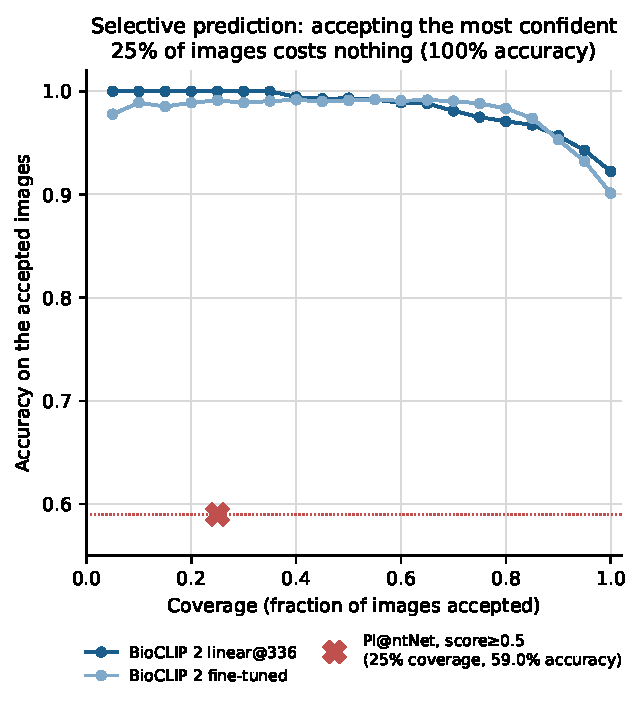
\includegraphics[width=\linewidth]{figures/Figure7_risk_coverage.pdf}
\caption{Risk-coverage curve for the specialist classifier and for the two general-purpose vision--language models, with the same curves for the Pl@ntNet service. Coverage is the fraction of images accepted at a given confidence threshold; risk is the error rate among accepted images.}
\label{fig:7}
\end{figure}

\setcounter{section}{7}

\setcounter{subsection}{4}

\subsection{Paired significance}\label{sec:7.5}

All systems saw the same images, so differences were tested with paired McNemar tests on the shared subset, with 95\% confidence intervals from bootstrap resampling (Table~\ref{tab:6}). The classifier beats every external system on the same images: +68.0 pp over Pl@ntNet, +60.3 pp over the stronger of the two vision--language models on the closed-set task, and +80.8 to +83.5 pp over the open-ended runs with leaked images removed; all p \textless{} 1e-16. Pl@ntNet in turn beats the open-ended vision--language models by +8.4 pp (p = 1e-5). Within our own results, the pairs that matter are reported where they belong, with the three-seed evidence in Section~\ref{sec:4}; Table~\ref{tab:6} lists the same comparisons from single-seed runs for completeness, and its footnote marks them as such.

\setcounter{section}{7}

\section{Error Structure}\label{sec:8}

RQ3 also asks how the systems fail, not only how often. This section compares the two systems by the structure of their mistakes rather than their rate: which species each system identifies at all, and how far each system's mistakes travel taxonomically.

\setcounter{section}{8}

\setcounter{subsection}{0}

\subsection{Species-level coverage}\label{sec:8.1}

Two species appear only once in the test split, \emph{Huperzia nanchuanensis} and \emph{H. sutchueniana}, so species-level counts are taken over the 148 species that have at least two test images; the accuracy figures still use all 902 images.

The classifier identifies all 148 species correctly at least once, and every one of them enters its top three at least once. Pl@ntNet never identifies 90 of the 148 (60.8\%), and 86 (58.1\%) never appear in its top three.

\setcounter{section}{8}

\setcounter{subsection}{1}

\subsection{Error taxonomy: cross-genus versus cross-family}\label{sec:8.2}

The classifier's errors are also taxonomically close, as Table~\ref{tab:8} shows. Of its 902 predictions, 47 (5.2\%) fall outside the true genus and 26 (2.9\%) outside the true family. Pl@ntNet's errors are not close: 446 (49.4\%) cross the genus boundary and 473 (52.4\%) cross the family boundary. Its worst single direction moves 188 of the 273 test images of Dryopteridaceae into Polypodiaceae, a different family, which is 68.9\% of that family's test images.

\begin{table}[tbp]
\centering
\begin{threeparttable}
\caption{Species-level coverage and error structure}
\label{tab:8}
\begin{tabularx}{\linewidth}{>{\raggedright\arraybackslash\hsize=1.0\hsize}X l >{\raggedright\arraybackslash\hsize=1.0\hsize}X}
\toprule
Metric & BioCLIP 2 linear@336 & Pl@ntNet \\
\midrule
Test images evaluated & 902 & 902 \\
Species represented (n $\geq$ 2 test images) & 148 & 148 \\
Never identified correctly & 0 (0.0\%) & 90 (60.8\%) \\
Never in the top-3 & 0 (0.0\%) & 86 (58.1\%) \\
Cross-genus errors & 47 (5.2\%) & 446 (49.4\%) \\
Cross-family errors & 26 (2.9\%) & 473 (52.4\%) \\
Largest single confusion direction & 3 images & 188 of 273 Dryopteridaceae images $\rightarrow$ Polypodiaceae \\
\bottomrule
\end{tabularx}
\begin{tablenotes}\footnotesize
\item Note. 'Species represented' counts species with $\geq$2 test images (148). The 902 test images cover 150 species in total; \emph{Huperzia nanchuanensis} and \emph{H. sutchueniana} contribute a single image each and are excluded only from the species-level counts, not from accuracy. 'Never in the top-3' is computed over each system's ranked candidate list (rank $\leq$ 3). Family errors are counted against the benchmark's PPG I family labels, using Pl@ntNet's own family field for its predictions.
\end{tablenotes}
\end{threeparttable}
\end{table}

The contrast is best stated as a ratio. Pl@ntNet's errors are eighteen times more likely to cross a family boundary than the classifier's (52.4\% against 2.9\% of all images). Looked at within each system's own errors, 63\% of the classifier's mistakes stay inside the correct family, whereas 69\% of Pl@ntNet's leave it.

\setcounter{section}{8}

\setcounter{subsection}{2}

\subsection{Per-family comparison}\label{sec:8.3}

Table~\ref{tab:7} gives family-level accuracy for the 28 families with at least five test images. The classifier falls below 0.60 on none of them, and its weakest family, Didymochlaenaceae, is represented by five images. Pl@ntNet scores exactly zero on eleven of the 28, and on those families the classifier ranges from 0.60 to 1.00.

\begin{table}[tbp]
\centering
\caption{Per-family accuracy, ours vs Pl@ntNet (n $\geq$ 5)}
\label{tab:7}
\resizebox{\linewidth}{!}{%
\begin{tabular}{lllll}
\toprule
Family & n & Ours (family acc.) & Pl@ntNet (family acc.) & Gap \\
\midrule
arthropteridaceae & 5 & 1.0 & 0.0 & 1.0 \\
athyriaceae & 10 & 0.9 & 0.0 & 0.9 \\
blechnaceae & 41 & 1.0 & 0.0 & 1.0 \\
cystopteridaceae & 10 & 1.0 & 0.0 & 1.0 \\
davalliaceae & 22 & 0.955 & 0.0 & 0.955 \\
didymochlaenaceae & 5 & 0.6 & 0.0 & 0.6 \\
grammitidaceae & 10 & 1.0 & 0.0 & 1.0 \\
lomariopsidaceae & 15 & 0.933 & 0.0 & 0.933 \\
nephrolepidaceae & 11 & 1.0 & 0.0 & 1.0 \\
pleurosoriopsidaceae & 5 & 1.0 & 0.0 & 1.0 \\
salviniaceae & 5 & 1.0 & 0.0 & 1.0 \\
dryopteridaceae & 273 & 0.974 & 0.07 & 0.905 \\
onocleaceae & 28 & 1.0 & 0.071 & 0.929 \\
lygodiaceae & 13 & 1.0 & 0.077 & 0.923 \\
hypodematiaceae & 18 & 0.944 & 0.111 & 0.833 \\
tectariaceae & 21 & 0.905 & 0.19 & 0.714 \\
marattiaceae & 15 & 0.867 & 0.333 & 0.533 \\
dennstaedtiaceae & 28 & 0.964 & 0.357 & 0.607 \\
gleicheniaceae & 28 & 0.964 & 0.464 & 0.5 \\
osmundaceae & 12 & 1.0 & 0.5 & 0.5 \\
aspleniaceae & 5 & 1.0 & 0.6 & 0.4 \\
hymenophyllaceae & 24 & 0.958 & 0.792 & 0.167 \\
polypodiaceae & 204 & 0.98 & 0.799 & 0.181 \\
ophioglossaceae & 24 & 1.0 & 0.833 & 0.167 \\
pteridaceae & 31 & 0.935 & 0.839 & 0.097 \\
lycopodiaceae & 24 & 1.0 & 0.958 & 0.042 \\
marsileaceae & 7 & 1.0 & 1.0 & 0.0 \\
psilotaceae & 8 & 1.0 & 1.0 & 0.0 \\
\bottomrule
\end{tabular}
}
\par\vspace{3pt}
\noindent\begin{minipage}{\linewidth}\footnotesize
Note. Pl@ntNet scores 0.000 on 11 families while ours stays 0.60--1.00 on every one of them.
\end{minipage}
\end{table}

The two systems do converge where Pl@ntNet's reference library is strong. On Polypodiaceae, its best-represented family, it reaches 0.799 against the classifier's 0.980; on Lycopodiaceae, 0.958 against 1.000. The gap is therefore not uniform. It is concentrated in the families where the API has no coverage at all.

Figure~\ref{fig:8} shows the decomposition and the per-family comparison together.

\begin{figure}[tbp]
\centering
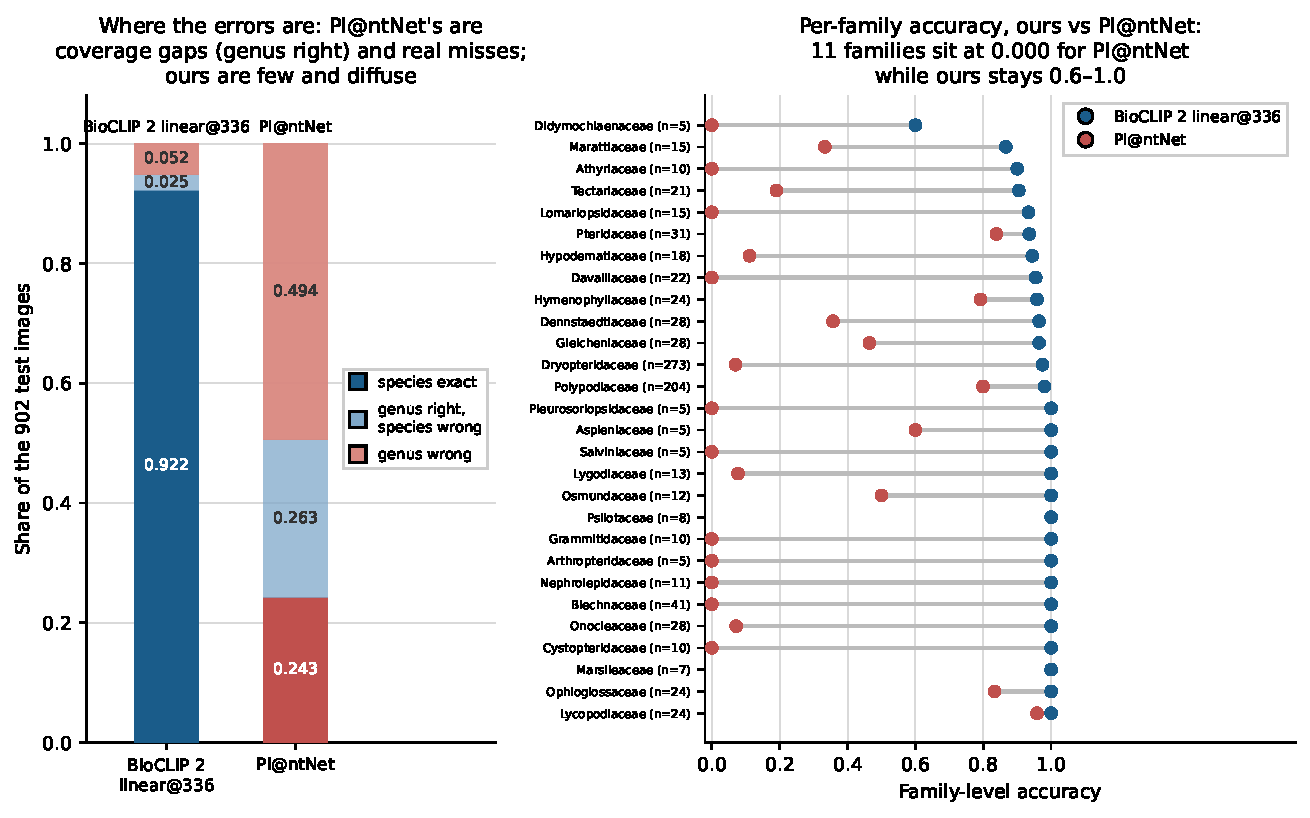
\includegraphics[width=\linewidth]{figures/Figure8_error_structure.pdf}
\caption{Error structure of the classifier and of the Pl@ntNet service. (a) Distribution of errors by taxonomic distance from the true species. (b) Per-family accuracy for the families with at least five test images. The classifier's remaining errors are confusions between congeneric species, whereas the service's errors frequently leave the family.}
\label{fig:8}
\end{figure}

\setcounter{section}{8}

\section{Open-Set Rejection}\label{sec:9}

RQ4 asks whether the model's own confidence can be used to automate decisions, and the first of the two decisions is open-set rejection. A closed-set classifier assigns every image to one of 152 species, including images that contain no fern at all. In monitoring that is the common case rather than the exception, since a pipeline receives whatever the camera or the contributor supplies. This section asks whether the model can be made to abstain.

\setcounter{section}{9}

\setcounter{subsection}{0}

\subsection{Negatives and the rejection score}\label{sec:9.1}

The 700 negatives described in Section~\ref{sec:3.6} are used as the positive class of the rejection problem: an image containing a horsetail, a moss, a cycad or a flowering plant should be refused. The rejection score is the maximum softmax probability of the closed-set classifier, which requires no additional training and no second model.

Section~\ref{sec:3.6} also noted the limitation that governs how these numbers should be read. The negative groups are not a random sample of what a deployment would see; the flowering-plant group is deliberately easy, and the cycad and palm groups are deliberately hard. Aggregate figures therefore describe behaviour on this set, and per-group rates are what carry over.

\setcounter{section}{9}

\setcounter{subsection}{1}

\subsection{Discrimination and per-group behaviour}\label{sec:9.2}

Table~\ref{tab:9} reports all seven trained models. The recipe of Section~\ref{sec:4} reaches an AUROC of 0.9666, with a true-positive rate of 0.9302 at a 10\% false-positive rate and 0.8426 at 5\%. Its mean confidence is 0.728 on positives against 0.168 on negatives, so the score separates the two populations by a wide margin and without a second decision stage.

\begin{table}[tbp]
\centering
\caption{Open-set rejection (700 negatives, 8 groups)}
\label{tab:9}
\resizebox{\linewidth}{!}{%
\begin{tabular}{lllllll}
\toprule
Model & AUROC & TPR@FPR5\% & TPR@FPR10\% & pos. conf. & neg. conf. & cycad rejection \\
\midrule
bioclip2\_ft & 0.9701 & 0.8182 & 0.8758 & 0.785 & 0.159 & 0.757 \\
bioclip2\_ft\_336 & 0.9666 & 0.8060 & 0.8858 & 0.813 & 0.185 & 0.743 \\
bioclip2\_linear\_336 & 0.9666 & 0.8426 & 0.9302 & 0.728 & 0.168 & 0.571 \\
bioclip2\_linear & 0.9634 & 0.8038 & 0.9047 & 0.708 & 0.167 & 0.600 \\
dinov2\_ft & 0.9425 & 0.6652 & 0.8204 & 0.657 & 0.137 & 0.686 \\
bioclip2\_ft\_hier & 0.9236 & 0.6175 & 0.7483 & 0.793 & 0.283 & 0.786 \\
dinov2\_linear\_336 & 0.9180 & 0.6386 & 0.7805 & 0.648 & 0.187 & 0.743 \\
\bottomrule
\end{tabular}
}
\par\vspace{3pt}
\noindent\begin{minipage}{\linewidth}\footnotesize
Note. max-softmax as the rejection score. The cycad group ('fern-like non-fern') is the weakest across every model.
\end{minipage}
\end{table}

Two qualifications belong with that ranking. The single highest AUROC in the set is 0.9701, from the 224 px fully fine-tuned model, which is not the recipe used elsewhere in this paper. The frozen probe ties the 336 px fine-tuned model on AUROC and is clearly ahead of it at the operating point that matters, with a true-positive rate of 0.9302 against 0.8858 at a 10\% false-positive rate. Rejection quality also tracks closed-set accuracy --- BioCLIP 2 models at 0.96 to 0.97, DINOv2 models at 0.92 to 0.94, the hierarchical head last at 0.9236 --- so closed-set accuracy, domain-transfer behaviour and rejection rank the seven models in the same order.

The per-group rates are more informative than the aggregate. At the 10\% false-positive operating point the model rejects 0.971 of horsetails, 0.971 of fungi, 0.971 of conifers, 0.948 of flowering plants, 0.943 of palms, 0.871 of out-of-scope lycopods and 0.857 of mosses and liverworts. The cycad group is the outlier at 0.571, and it is the outlier in every model tested, ranging from 0.57 to 0.79 across all seven. Palm is second hardest. What the two hard groups share is pinnate foliage, which converges on fern morphology in a single photograph. The other six groups, which include taxa with no fern-like resemblance at all, are rejected at 0.85 or better.

Combining rejection with the selective policy of Section~\ref{sec:7.4} gives a two-stage rule: reject anything whose maximum probability falls below the threshold, then accept the most confident fraction of what remains.

\setcounter{section}{9}

\section{Discussion}\label{sec:10}

\setcounter{section}{10}

\setcounter{subsection}{0}

\subsection{Why mixed-domain and mixed-geography evaluation overstates capability}\label{sec:10.1}

Each of the three assumptions set out in the Introduction has now been tested, and each fails. A pooled accuracy of 0.9139 describes neither image regime: the same model reaches 0.9198 on herbarium sheets and 0.9250 on field photographs when both are in training, while crossing the regimes costs 8.6 to 48.1 pp. A benchmark number is therefore a property of its composition and not only of the model --- change the specimen share of the test set and the reported accuracy changes, without anything about identification having changed.

Geographic provenance is not exchangeable either, and its cost is not a constant. Holding out Taiwan, China costs 39.8 pp; holding out Vietnam costs 3.6 pp, against the same model and the same recipe. What separates the two is not distance or continent, both being in Asia, but whether the target species keep training images outside the held-out region --- a Spearman correlation of 0.48 across seven countries, weak as a fitted relationship and decisive as a contrast between well-supported and poorly-supported regions.

The third assumption fails in the most consequential way. For the two vision--language models tested, apparent accuracy on herbarium material is largely an artefact of readable labels: their morphological accuracy, measured on images whose species name is not machine-readable, is 0.0825 to 0.1092. The asymmetries behind these verdicts, and the mechanisms they suggest, are taken up in Section~\ref{sec:10.2}.

\setcounter{section}{10}

\setcounter{subsection}{1}

\subsection{A mechanistic account}\label{sec:10.2}

Each verdict above admits a candidate mechanism. Three are set out here; none is proven, each makes a prediction testable without re-running these experiments, and each is stated so that it can fail.

The asymmetry between the crossing directions runs against the usual expectation: training on field photographs and testing on herbarium sheets costs 48.1 pp, the reverse only 19.9 pp, whereas if a sheet were a narrower sample of the field distribution, broader-to-narrower should be the cheaper direction. A character-based account explains the reversal. The two regimes do not show the same plant: a pressed sheet is photographed on both surfaces and exposes the ventral characters on which fern determination has always relied --- sorus position and form, indusium, indument, rhizome scales --- whereas a field photograph shows habit and substrate but rarely the underside of the frond. A model trained in one regime reads the characters that regime exposes and falls back on gross morphology when they are absent, so the cost of a crossing is set by how much of the diagnostic character set survives it. The prediction is that transfer cost should be largest for species separated by ventral or sporangial characters and smallest for species separable by habit; this benchmark tests it only coarsely, and it is testable sharply on new data by scoring the same species under controlled character occlusion.

The geographic result has a mechanism of a different kind. The loss does not follow from where the held-out region is: the two extremes are both in Asia, and what separates them is the share of each species' training support outside the region. A two-term account follows. The first term is coverage --- a holdout removes instances, and the loss scales with the share of a species' image pool that was removed, which is why the association with out-of-region support is positive across seven countries even though it is weak. The second is composition --- each region's test set carries its own specimen share, and the domain axis costs up to 48 pp, so part of every holdout drop is a domain effect in disguise. The first term is one a deployment can act on; the second is one an evaluation has to control, and no experiment here separates them. That coverage dominates is consistent with the biases documented for plant occurrence records \citep{meyer2016} and with the scarcity of species-level records in under-surveyed floras \citep{scheffers2012}, and it relocates the geographic problem from cartography to data acquisition.

The third mechanism concerns the external models and has the widest reach. For a general-purpose vision--language model choosing among 152 species, the printed label on a sheet is a cue of higher reliability and lower variance than morphological inference; where the label is available, reading it maximises expected accuracy, so a model evaluated on herbarium material can appear competent while doing something else entirely. The domain asymmetry is the fingerprint of that shortcut: the model that reaches 0.379 on sheets reaches 0.069 on field photographs, and the subsets differ in text availability rather than difficulty. This yields a diagnostic that costs nothing to apply --- a domain-asymmetric accuracy profile across herbarium and field material is evidence of reading until shown otherwise --- and predicts that masking label regions should erase most of the apparent herbarium competence.

Two observations sit outside this account, recorded as open questions. The first is the zero-shot result: with no task-specific training, BioCLIP 2 reaches 0.6829 at species level over 152 classes --- orders of magnitude above chance and well below the trained recipe --- so biological pretraining encodes species-level morphology to a degree no experiment here was designed to measure; what such a model gets right and wrong without training, and whether its errors are taxonomically structured, is answerable on this benchmark and unanswered. The second is a single region: Russia has the second-thinnest out-of-region support of the eight holdouts, at 0.15, and loses only 5.6 pp, which the coverage term does not predict. The holdout is small (54 test images), so the estimate is noisy, but it is the one case in which the mechanism fails in the wrong direction, and the annotations this benchmark carries do not explain it.

\setcounter{section}{10}

\setcounter{subsection}{2}

\subsection{Deployment: selective prediction and a data-acquisition checklist}\label{sec:10.3}

The practical question a monitoring programme faces is not which model is more accurate but how to use one safely. The first mechanism is rejection. A maximum-softmax threshold on the frozen probe gives an AUROC of 0.9666 and rejects 85 to 97\% of out-of-scope images at a 10\% false-positive rate for most negative groups, at no additional training cost. The exception is fern-like foliage: cycads are rejected 57\% of the time, a weakness shared by every model tested, so a pipeline should route fern-like non-ferns to human review rather than assume rejection handles them.

The second is selective acceptance, which the classifier's under-confidence makes safe: accepting the most confident quarter of images yields 100\% accuracy, and accepting 85\% still holds 0.967. The contrast with Pl@ntNet is not the one the standard summary predicts. Pl@ntNet has the lower expected calibration error of the two systems (0.090 against 0.195) and is the less usable of the two, because its most confident bin claims 0.943 and delivers 0.683. The summary statistic ranks the two systems in the opposite order to their decision-relevant behaviour: what a pipeline needs to know is not how large the calibration error is but which way it points.

Both profiles have a mechanism the literature does not predict. \citet{guo2017} report over-confidence as the norm in modern networks, yet the frozen probe here is under-confident in every bin --- a property of the linear head, which never learns to sharpen (full fine-tuning reaches an expected calibration error of 0.095 against 0.195), not of biological pretraining.

The two systems also fail in structurally different ways (Section~\ref{sec:8}): the classifier's errors stay taxonomically close, Pl@ntNet's cross family boundaries and concentrate exactly in the families where the API has no coverage at all --- for a downstream user who can tolerate a wrong species but not a wrong family, that contrast matters more than the accuracy gap.

These results support a deployment recipe, but they also imply a data requirement, which is the more transferable conclusion: each target species should retain more than five training images from outside the deployment region, and if the intake will contain pressed or flattened material as well as living plants, both regimes must appear in training. Neither requirement is met by collecting more images from the deployment site alone.

\setcounter{section}{10}

\setcounter{subsection}{3}

\subsection{Relationship to related work}\label{sec:10.4}

The closest agreement in the literature is with evaluations of plant identification applications --- agreement about a condition rather than a number. \citet{partel2021}, \citet{rzanny2024} and \citet{mader2021} report high accuracy in well-sampled settings; our results agree on their own terms and locate the condition they rest on: Pl@ntNet reaches 0.799 on its best-covered family and exactly zero on eleven of the 28 families with at least five test images. The accuracy those studies measure is a property of referential coverage before it is a property of the model, and \citet{garcin2021} named the two properties that matter: long-tailed coverage and label ambiguity.

A literature reaching the opposite conclusion about the same tools is the point of disagreement. \citet{campbell2023}, \citet{hart2023} and \citet{long2023} find the applications unreliable, sensitive to image framing and to who scores the outcome, and attribute the failure to the evaluation protocol; their remedies are procedural. The domain split here shows a failure no scoring convention repairs --- 0.004 on herbarium sheets against 0.341 on field photographs, from a system whose ranking quality is not in question. A coverage failure is not a protocol failure.

Table~\ref{tab:10} compares this benchmark with the three others a reader of this literature will have in mind. Pl@ntNet-300K \citep{garcin2021} is the reference plant image dataset: 306,146 field images over 1,081 species, difficult by design through a long-tailed class distribution and label ambiguity. PlantCLEF 2025 \citep{martellucci2025} shifts the difficulty to acquisition, training on about 1.4 million close-up images and testing on 2,105 expert-annotated quadrat views; Section~\ref{sec:5} puts a number on the component their design contains. The New Guinea orchid benchmark \citep{saputra2026} confronts a data-poor flora with a two-stage genus-then-retrieval system. None of the three annotates image domain, performs a geographic holdout, or ships labelled negatives; this benchmark was built to carry all three, which is what makes the measurements of Sections~\ref{sec:5} to~\ref{sec:9} possible on one image set with one model.

\begin{table}[tbp]
\centering
\caption{Comparison with existing plant and fern identification benchmarks}
\label{tab:10}
\resizebox{\linewidth}{!}{%
\begin{tabular}{lllllll}
\toprule
Benchmark & Scale (images) & Taxa & Domain annotation & Geography annotation & Open-set negatives & Protocol \\
\midrule
NGOI benchmark (New Guinea orchids; Saputra et al. 2026, arXiv:2609.24064) & 16,701 photographs & 1,350 spp. / 120 genera (Orchidaceae, New Guinea) & no (field photographs only) & no (single island flora) & no (but distance-based open-set gate for unseen genera, AUROC 0.958) & fixed species-stratified partition; two-stage genus + FAISS species retrieval \\
Pl@ntNet-300K & 306,146 (244k/31k/31k) & 1,081 spp. (French flora) & no (field photographs only) & no & no & random train/val/test split \\
PlantCLEF 2025 & 2,105 test quadrats + \textasciitilde{}1.4M train single-plant images & \textasciitilde{}400 spp. & no (field imagery only) & no & no & split by acquisition mode (close-up vs quadrat) \\
This benchmark & 5,969 (4,185/882/902) & 152 spp. / 30 families & yes (field / herbarium) & yes (country, 80 values) & yes (700 images / 8 groups) & group-aware by observation; domain, source and geography holdouts \\
\bottomrule
\end{tabular}
}
\par\vspace{3pt}
\noindent\begin{minipage}{\linewidth}\footnotesize
Note. Sources: \citet{garcin2021} for Pl@ntNet-300K; \citet{martellucci2025} for PlantCLEF 2025; Saputra et al. (2026, arXiv:2609.24064) for the New Guinea Orchid Identifier (NGOI) benchmark.
\end{minipage}
\end{table}

On the design side, the orchid benchmark is the closest work: they evaluate genus-level identification after fine-tuning and report that general-purpose self-supervision beats biological pretraining, whereas we evaluate species-level identification with a frozen probe and find the opposite. The mechanism proposed in Section~\ref{sec:10.2} reconciles the two and turns the disagreement into a prediction --- biological pretraining carries diagnostic characters that a linear head cannot re-learn, so pretraining domain dominates while adaptation is frozen, whereas a fine-tuned trunk can recover what its pretraining lacks. Our numbers support the first half, the backbone gap of +7.1 pp being an order of magnitude larger than the adaptation-mode gap of +0.55 pp, but this benchmark tests one cell of the interaction and not the other. Work adapting a global plant model to new imagery shows the other end, what adaptation can recover (Espitalier et al., 2025, this journal); the cost measured here bounds the benefit it can be chasing.

The herbarium literature has called for measurement of exactly this kind: systematic reviews name cross-domain identification as an open problem \citep{hussein2022} and give explicit attention to label text and open-set conditions \citep{guo2025}. Where those reviews describe label text as unsettled, the audit here suggests it is dominant, and the reading shortcut of Section~\ref{sec:10.2} is a candidate explanation. In earlier work we audited five vision--language models on a much smaller 155-image set; the present audit re-runs on the full benchmark with text-leakage control, and the two sets of numbers are not comparable, because image sets, prompts and leakage treatment all differ.

The methodological instruments come from outside ecology: selective classification supplies the risk-coverage curve \citep{geifman2017}, the calibration literature explains over-confidence \citep{guo2017}, and open-set recognition has its own evaluation \citep{geng2020,yang2024,wang2023}. Botanical benchmarks have adopted neither. Applying both exposes the finding that matters for deployment: the specialist model here is worse calibrated than the commercial API in absolute terms, yet is the only one of the two whose confidence supports automated acceptance, because its errors point in the safe direction.

\setcounter{section}{10}

\setcounter{subsection}{4}

\subsection{Limitations}\label{sec:10.5}

Six limitations bound what these results support. The leave-one-region-out experiments confound removing a region with removing data: the per-holdout training sets differ in size from 2,860 to 4,088 images, and the two effects cannot be separated from these runs alone. Each country's test set also differs in image-domain composition, from 2\% specimens for Taiwan, China to 81\% for Thailand, so a holdout difference carries a domain component as well as a geographic one, and no experiment here estimates the interaction. The small holdouts have wide intervals --- Vietnam has 28 test images and Thailand 31, roughly $\pm$14 pp --- so the argument rests on the contrast between the China-region holdouts and the well-supported ones rather than on any single country. The backbone comparison covers one pair, chosen to isolate pretraining data; a conclusion about pretraining domain drawn from two models is a claim about those two models. The mechanisms of Section~\ref{sec:10.2} are interpretations, not measurements --- consistent with the direction and size of the effects but not tested by them --- and no claim in Sections~\ref{sec:4} to~\ref{sec:9} depends on them. A sixth limit applies to reuse: the openly licensed 24\% over-represents herbarium material (63.3\% specimens against 28.0\% in the full set), so the field-side results and the geographic holdouts cannot be reproduced from the released images alone (Section~\ref{sec:12}). Finally, the benchmark is a snapshot without a time axis: phenological variation, from sterile fronds to spore-bearing maturity, and extreme juvenile stages are represented only incidentally, and a monitoring programme that observes a site across seasons will meet variation this benchmark does not score.

\setcounter{section}{10}

\setcounter{subsection}{5}

\subsection{Future work}\label{sec:10.6}

Three directions follow directly, and the first two test the mechanisms of Section~\ref{sec:10.2} rather than extend the measurements. Recovering coordinates for the occurrence records would replace the region-level analysis of Section~\ref{sec:6} with a per-species distance to the nearest training occurrence, though the country field is not sufficient and the reconstruction would need verification against the source records. Second, the label-text problem invites a controlled experiment rather than an audit: masking or removing label regions and re-measuring the models would separate reading from identification more sharply than excluding leaky images can. Third, the confusions that remain are morphological; attention maps for the errors in Section~\ref{sec:8} would show whether the classifier is using venation and sorus characters or something incidental, and would clarify why fern-like foliage defeats rejection in every model tested.

Two further directions follow from the open questions in Section~\ref{sec:10.2}: the character-based account predicts that transfer cost varies with which diagnostic characters a species' separation rests on, testable by scoring transfer per family and by controlled character occlusion; and the zero-shot result, 0.6829 with no training, raises the question of how much species-level morphology biological pretraining already encodes and what structure its errors have.

\setcounter{section}{10}

\section{Conclusion}\label{sec:11}

The question this paper opened with was whether a benchmark accuracy can serve as an estimate of field performance. On this benchmark the answer is no, and the distance between the two is measurable rather than mysterious. One model trained on both image regimes reaches 91.9\% on herbarium sheets and 92.5\% on field photographs; separate the regimes between training and test and accuracy falls to 42 to 65\%; withhold one region and a single step costs 39.8 percentage points. None of those losses appears in the number a conventionally split benchmark reports, and each is large enough to reverse a ranking. The three assumptions that keep them hidden have each been tested here, and each fails.

Against the four questions posed in Section~\ref{sec:2}: biology-pretrained features with a frozen trunk and a linear head at 336 px are the best recipe, at 91.4 $\pm$ 0.7\% over three seeds, statistically indistinguishable from full fine-tuning and +7.1 $\pm$ 1.0 pp ahead of a general-purpose self-supervised backbone (RQ1). Withholding image domain, data source or region costs 8.6 to 48.1 pp and 3.6 to 39.8 pp, measured against baselines on the same images (RQ2). A specialist API reaches 0.2428 at species level and never identifies 60.8\% of the benchmark's species, while two general-purpose vision--language models reach 24 to 32\% closed-set and 8.3 to 10.9\% open-ended once machine-readable names are removed (RQ3). The specialist model's own confidence supports automated decisions --- rejecting 85 to 97\% of out-of-scope images at a 10\% false-positive rate and giving 100\% accuracy on the most confident quarter --- where the API's does not (RQ4).

What the work adds is the measurement whose absence has kept this question open --- a measurement rather than a model --- with three consequences that outlive the benchmark. A pooled accuracy is a property of the composition of the test set as much as of the model, so the number moves when the specimen share moves, with nothing about identification having changed. The confound that most threatens the herbarium literature is now quantified rather than suspected, and it is large enough to reorder two systems. And the losses are attributable to identifiable factors --- training support and image regime --- which is what makes them actionable.

The timing matters because both conditions the audit identifies are expanding at once. Institutional digitisation is converting herbaria into image collections faster than expert review can follow, every sheet carries its species name in machine-readable print, and general-purpose vision--language models are being pointed at exactly that material. An evaluation that does not separate reading from identification will report competence that does not exist --- and the diagnostic proposed in Section~\ref{sec:10.2}, a domain-asymmetric accuracy profile across the two regimes, can be run on any existing result at no cost.

For a monitoring programme the practical reading is a checklist rather than a model choice: each target species should retain training images from elsewhere, and if the intake will contain pressed or flattened material as well as living plants, both regimes must appear in training. Neither is met by collecting more images from the deployment site alone.

Two boundaries qualify the above. The backbone comparison covers one pair of models, and the mechanisms of Section~\ref{sec:10.2} are frameworks that later work can confirm or discard rather than measurements; the numbers that answer the four questions would change first on another image set. The directions that follow --- coordinates in place of regions, masked labels in place of exclusion, per-family transfer in place of aggregates --- are set out in Section~\ref{sec:10.6}, together with the two observations this benchmark can explain and this paper does not.

\setcounter{section}{11}

\section{Data and Code Availability}\label{sec:12}

The benchmark is released as metadata plus code, and the openly licensed part of it as images as well. The package contains: the manifest of the 5,969-image balanced benchmark (\texttt{manifest\_balanced.\allowbreak{}csv}, 31 fields per image, including image domain, source, country, taxonomy, licence, rights holder, source identifiers and URLs, and the split group key) and of the 6,237-image pre-balancing pool; the 4,185/882/902 splits and the seven evaluation subsets of Sections~\ref{sec:5} and~\ref{sec:6}; the 700-image open-set negative manifest; the 1,432 (24.0\%) openly licensed images as a single archive with a per-image licence file; and all code under an open-source licence, which rebuilds the manifests, trains and evaluates every model reported here, and regenerates Tables 1--10 and Figures 3--8, with per-run configurations, metrics and per-image predictions for the 37 experimental runs. The repository documentation describes each artefact, the licence layers and the reproduction environment in full.

Every image carries the licence recorded by its source platform: CC0, public domain, CC BY and CC BY-SA are classed as redistributable, and the two NonCommercial variants --- the only reason any image is withheld --- account for all 4,537 restricted records. The code is released under the MIT licence, the manifests and derived metadata under CC BY 4.0; no image is relicensed.

The open subset is not a random 24\% of the benchmark, and the skew limits what a reader can reproduce from the images alone. The released images are 63.3\% herbarium specimens, against 28.0\% in the benchmark as a whole, because institutional digitisation releases sheets under permissive terms (54.3\% of GBIF specimen images) while volunteer field photographs are predominantly CC BY-NC (10.2\% of iNaturalist images). Only 216 of the 902 test images (23.9\%) can be redistributed --- 69 of 640 field images against 147 of 262 specimen images --- so a reader with the open archive can reproduce the specimen-side results and the specimen-to-field direction of Section~\ref{sec:5}, but not the field-side experiments or the geographic holdouts. The open archive should not be used as a stand-alone field-identification benchmark, and accuracies recomputed on it will not match the numbers in this paper.

Three details affect exact reproduction and are recorded in the released configuration files. The label space is rebuilt from the filtered training split, a correction disclosed in Section~\ref{sec:5.4}. Seed standard deviations are population standard deviations (ddof = 0). Fine-tuning is not bit-deterministic (about $\pm$0.2 pp per re-run), which is why the recipe comparison is reported as a three-seed mean; the frozen probe reproduces exactly.

\#\# Data availability statement

\begin{quote}
The image manifests, split files, evaluation subsets and open-set negative manifest, the source code, the per-run configurations and metrics, and the per-image predictions are openly available at [repository URL]. Of the 5,969 images in the benchmark, 1,432 (24.0\%) are published under their original Creative Commons licences, together with a per-image licence and attribution file. The remaining 4,537 images are licensed CC BY-NC or CC BY-NC-SA and are therefore not redistributed. They are fully described in the manifest, which records the licence, rights holder, source record identifier and source URL for each image. The dataset can be reconstructed from iNaturalist and GBIF subject to their terms. The openly licensed subset covers 216 of the 902 test images and over-represents herbarium material relative to the benchmark as a whole. The limits this places on independent reproduction are set out in Section~\ref{sec:12}. Archived versions of the manifests and code are deposited at [DOI].
\end{quote}

\section*{Declarations}
\subsection*{CRediT authorship contribution statement}
\textbf{Zihao Huang}: Conceptualization, Data curation, Formal analysis,
Investigation, Methodology, Software, Visualization, Writing -- original draft.
\textbf{Yan Chen}: Data curation, Funding acquisition, Resources, Validation,
Writing -- review \& editing. \textbf{Yeming You}: Resources, Validation,
Writing -- review \& editing. \textbf{Qi Zhang}: Investigation,
Writing -- review \& editing. \textbf{Kai Su}: Conceptualization, Funding
acquisition, Supervision, Validation, Writing -- review \& editing.
\subsection*{Funding}
This work was supported by the Guangxi Key Technologies R\&D Program
(AB25069151), the Open Project Program of Guangxi Key Laboratory of Digital
Infrastructure (Grant No. GXDINBC202501), the National Natural Science
Foundation of China (Grant No. 72461001), and the Guangxi Natural Science
Foundation (Grant No. 2025GXNSFAA069138).
\subsection*{Declaration of competing interests}
The authors declare that they have no known competing financial interests or
personal relationships that could have appeared to influence the work reported
in this paper.
\subsection*{Declaration on the use of generative AI in scientific writing}
During the preparation of this work, the authors used generative AI tools to
assist in drafting an initial Chinese-language version of the manuscript,
translating content into English, and improving English-language expression.
The authors reviewed and edited the output as needed and take full
responsibility for the content of the published article.
\subsection*{Data availability statement}
See \texttt{11\_data\_code\_availability.\allowbreak{}md} for the full statement, including the
repository URL and the archive DOI, both of which are still to be filled in.
---

% Elsevier places the reference list after the declarations.
\begin{thebibliography}{99}
\bibitem[Bai et al.(2025)]{bai2025} Qwen3-VL technical report. \emph{arXiv preprint}, arXiv:2511.21631.
\bibitem[Campbell et al.(2023)]{campbell2023} A repeatable scoring system for assessing Smartphone applications ability to identify herbaceous plants. \emph{PLOS ONE}, 18(4), e0283386.
\bibitem[Espitalier et al.(2025)]{espitalier2025} Adapting a global plant identification model to detect invasive alien plant species in high-resolution road side images. \emph{Ecological Informatics}, 89, 103129.
\bibitem[Garcin et al.(2021)]{garcin2021} Pl@ntNet-300K: A plant image dataset with high label ambiguity and a long-tailed distribution. \emph{Proceedings of the Neural Information Processing Systems Track on Datasets and Benchmarks}, 1.
\bibitem[GBIF Secretariat(2023)]{gbifsecretariat2023} \emph{GBIF occurrence data and API documentation}. Global Biodiversity Information Facility.
\bibitem[Geifman et al.(2017)]{geifman2017} Selective classification for deep neural networks. \emph{Advances in Neural Information Processing Systems}, 30, 4878--4887.
\bibitem[Geng et al.(2020)]{geng2020} Recent advances in open set recognition: A survey. \emph{IEEE Transactions on Pattern Analysis and Machine Intelligence}, 43(10), 3614--3631.
\bibitem[Goëau et al.(2017)]{goeau2017} Plant identification based on noisy web data: The amazing performance of deep learning (LifeCLEF 2017). \emph{CLEF 2017 Working Notes}.
\bibitem[Gu et al.(2025)]{gu2025} BioCLIP 2: Emergent properties from scaling hierarchical contrastive learning. \emph{Advances in Neural Information Processing Systems}, 38, 102778--102811.
\bibitem[Guo et al.(2017)]{guo2017} On calibration of modern neural networks. \emph{Proceedings of the 34th International Conference on Machine Learning}, 1321--1330.
\bibitem[Guo et al.(2025)]{guo2025} A review of artificial intelligence in herbarium specimen image analysis. \emph{Artificial Intelligence Review}, 58, 402.
\bibitem[Hart et al.(2023)]{hart2023} Assessing the accuracy of free automated plant identification applications. \emph{People and Nature}, 5(3), 929--937.
\bibitem[Hussein et al.(2022)]{hussein2022} Applications of computer vision and machine learning techniques for digitized herbarium specimens: A systematic literature review. \emph{Ecological Informatics}, 69, 101641.
\bibitem[Ilharco et al.(2021)]{ilharco2021} \emph{OpenCLIP}. Zenodo.
\bibitem[Joly et al.(2014)]{joly2014} Interactive plant identification based on social image data. \emph{Ecological Informatics}, 23, 22--34.
\bibitem[Kahl et al.(2021)]{kahl2021} BirdNET: A deep learning solution for avian diversity monitoring. \emph{Ecological Informatics}, 61, 101236.
\bibitem[Kumar et al.(2012)]{kumar2012} Leafsnap: A computer vision system for automatic plant species identification. \emph{Proceedings of the European Conference on Computer Vision}, 502--516.
\bibitem[Long et al.(2023)]{long2023} Plant identification applications do not reliably identify toxic and edible plants in the American Midwest. \emph{Clinical Toxicology}, 61(7), 524--528.
\bibitem[Mac Aodha et al.(2019)]{macaodha2019} Presence-only geographical priors for fine-grained image classification. \emph{Proceedings of the IEEE/CVF International Conference on Computer Vision}, 9596--9606.
\bibitem[Martellucci et al.(2025)]{martellucci2025} Overview of PlantCLEF 2025: Multi-species plant identification in vegetation quadrat images. \emph{CLEF 2025 Working Notes}.
\bibitem[Mäder et al.(2021)]{mader2021} The Flora Incognita app: Interactive plant species identification. \emph{Methods in Ecology and Evolution}, 12(7), 1335--1342.
\bibitem[Meyer et al.(2016)]{meyer2016} Multidimensional biases, gaps and uncertainties in global plant occurrence information. \emph{Ecology Letters}, 19(8), 992--1006.
\bibitem[Oquab et al.(2024)]{oquab2024} DINOv2: Learning robust visual features without supervision. \emph{Transactions on Machine Learning Research}.
\bibitem[Page and C(2002)]{page2002} Ecological strategies in fern evolution: A neopteridological overview. \emph{Review of Palaeobotany and Palynology}, 119(1--2), 1--33.
\bibitem[PPG I(2016)]{ppgi2016} A community-derived classification for extant lycophytes and ferns. \emph{Journal of Systematics and Evolution}, 54(6), 563--603.
\bibitem[Pärtel et al.(2021)]{partel2021} Plant image identification application demonstrates high accuracy in Northern Europe. \emph{AoB PLANTS}, 13(4), plab050.
\bibitem[Radford et al.(2021)]{radford2021} Learning transferable visual models from natural language supervision. \emph{Proceedings of the 38th International Conference on Machine Learning}, 8748--8763.
\bibitem[Rzanny et al.(2024)]{rzanny2024} More than rapid identification---Free plant identification apps can also be highly accurate. \emph{People and Nature}, 6(6), 2178--2181.
\bibitem[Saputra et al.(2026)]{saputra2026} Vision Transformers versus convolutional neural networks for fine-grained orchid genus identification in a species-rich, data-poor flora: A controlled benchmark on the Orchidaceae of New Guinea. \emph{arXiv preprint}, arXiv:2609.24064.
\bibitem[Scheffers et al.(2012)]{scheffers2012} What we know and don't know about Earth's missing biodiversity. \emph{Trends in Ecology \& Evolution}, 27(9), 501--510.
\bibitem[Stevens et al.(2024)]{stevens2024} BioCLIP: A vision foundation model for the tree of life. \emph{Proceedings of the IEEE/CVF Conference on Computer Vision and Pattern Recognition}, 19412--19424.
\bibitem[Tuia et al.(2022)]{tuia2022} Perspectives in machine learning for wildlife conservation. \emph{Nature Communications}, 13, 792.
\bibitem[Van Horn et al.(2018)]{vanhorn2018} The iNaturalist species classification and detection dataset. \emph{Proceedings of the IEEE Conference on Computer Vision and Pattern Recognition}, 8769--8778.
\bibitem[Wäldchen et al.(2018)]{waldchen2018} Automated plant species identification: Trends and future directions. \emph{PLOS Computational Biology}, 14(4), e1005993.
\bibitem[Wang et al.(2023)]{wang2023} Can multi-label classification networks know what they do not know? \emph{Advances in Neural Information Processing Systems}, 36.
\bibitem[Yang et al.(2024)]{yang2024} Generalized out-of-distribution detection: A survey. \emph{International Journal of Computer Vision}, 132(12), 5635--5662.
\end{thebibliography}

\end{document}
